\documentclass[a4paper]{scrreprt}

\usepackage[ngerman]{babel}
\usepackage[utf8]{inputenc}
\usepackage[T1]{fontenc}
\usepackage{ae}
\usepackage[bookmarks, bookmarksnumbered]{hyperref}
\usepackage{tabularx}
\usepackage{graphicx}
\usepackage{csquotes}
\usepackage{verbatim}
\usepackage[nonumberlist, toc, section]{glossaries}
\usepackage[german]{fancyref}

\makeglossaries

\newglossaryentry{Produkt}
{
name=Produkt,
plural=Produkte,
description={Das von uns gelieferte Softwaresystem.}
}

\newglossaryentry{Webbrowser}
{
name=Webbrowser,
plural=Webbrowser,
description={Für dieses Produkt wird nur auf Google Chrome und Mozilla Firefox hin entwickelt.}
}

\newglossaryentry{Spiel}
{
name=Spiel,
plural=Spiele,
description={Ein Spiel ist eine Instanz eines \Gls{Spielmodus}. Ein Spiel hat das Ziel, das Wissen des Spielers zu nutzen, um die Merkmalsauswahl für Machine Learning zu unterstützen.}
}
\newglossaryentry{Spielmodus}
{
name=Spielmodus,
plural=Spielmodi,
description={Ein Spielmodus ist eine definierte Art und Weise, die Merkmalsauswahl durchzuführen. Standardmäßig gibt es die Spielmodi \Gls{Matrix Select} und \Gls{Binar Select}}.
}
\newglossaryentry{Matrix Select}
{
name=Matrix Select,
plural=Matrix Select,
description={Matrix Select ist ein \Gls{Spielmodus}, in dem ein \Gls{Spieler} eine Matrix, bestehend aus einer vom \Gls{Organisator} festgelegten Anzahl an Merkmalen, angezeigt bekommt und davon eine Teilmenge auswählt, die die Merkmale enthält, die für das Machine Learning am wichtigsten sind. Die Größe der Teilmenge wird ebenfalls vom Organisator in den Spieleinstellungen festgelegt. Eine Runde besteht aus genau einer Matrix von Merkmalen.}
}
\newglossaryentry{Binar Select}
{
name=Binär Select,
plural=Binär Select,
description={Binär Select ist ein \Gls{Spielmodus}, in dem ein \Gls{Spieler} genau zwei Merkmale angezeigt bekommt, diese vergleicht und das Merkmal auswählt, welches für das Machine Learning wichtiger ist. Eine Runde besteht aus fünf Vergleichen.}
}

\newglossaryentry{Spieler}
{
name=Spieler,
plural=Spieler,
description={Ein Nutzer, welcher an einem Spiel teilnimmt. Meist ist dies ein Angestellter des Betriebs.}
}

\newglossaryentry{Spieleinstellungen}
{
name=Spieleinstellungen,
plural=Spieleinstellungen,
description={Einstellungen für ein Spiel umfassen: die Merkmale, welche ausgewählt werden soll, die Art des Spiels, die teilnehmenden Spieler, Endbedingungen des Spiels.}
}
\newglossaryentry{Organisator}
{
name=Organisator,
plural=Organisatoren,
description={Ein Organisator ist ein Nutzer, der neue Spiele erstellt und die Ergebnisse von diesen ausliest.}
}
\newglossaryentry{Achievement}
{
name=Achievement,
plural=Achievements,
description={Ein Ziel oder eine Errungenschaft, welche den Spieler motiviert, weiterzuspielen.}
}
\newglossaryentry{Administrator}
{
name=Administrator,
plural=Administratoren,
description={Die Person, welche das System installiert und den Nutzern zur Verfügung stellt. Sie verwaltet den \Gls{Spiele-Server}.}
}
\newglossaryentry{Spiele-Server}
{
name=Spiele-Server,
plural=Spiele-Server,
description={Ein Computer, welcher der Verwaltung von CS:Select dient und eine Internetanbindung hat.}
}
\newglossaryentry{ML-Server}
{
name=Machine-Learning-Server,
description={Ein Server, der nicht Bestandteil des Produktes ist, jedoch benötigt wird, um die Funktionalität des Produktes herzustellen.}
}

\newglossaryentry{Datensatz}
{
    name=Datensatz,
    description={Die Menge an Features, die ein Machine Learning Modell zur Verfügung hat. Zu jedem Feature gehört noch eine Beschreibung und zwei Bilder.}
}
\begin{document}

    \title{Pflichtenheft CS-Select}
    \author{Luca Springer, Alexander Linder, Julian Dinh, Nicholas Bieker,\\ Bendix Sonnenberg}
    \maketitle

    % Platzierung des Inhaltsverzeichnisses
    \tableofcontents

    \chapter{Einleitung}
        In der heutigen Zeit wird Machine Learning in immer mehr Organisationen eingesetzt, um vorhersagende Systeme zu entwickeln.
        Das Problem dabei ist: Es werden Werte für viele Merkmale aufgenommen, aber die Personen, welche das Netzwerk trainieren, haben meist kaum Wissen über die Zusammenhänge dieser Daten.
        Das sogenannte Domänenwissen liegt oft bei den Personen, welche den gesamten Tag z.B. an der Produktionslinie verbringen. Einige der Merkmale sind vielleicht offensichtlich nutzlos
        für das, was mit dem Machine Learning vorhergesagt werden soll. \footnote{Zum Beispiel ist die Außentemperatur nicht sehr aussagekräftig, wenn es um die Geschwindigkeit eines fallenden
        Balls geht. Aber woher soll das denn der Computer wissen.} Es gibt bereits verschiedene Algorithmen, die dies übernehmen, aber diese sind meist zu langsam oder zu ineffizient.
        \footnote{\href{https://de.wikipedia.org/wiki/Feature\_Subset\_Selection}{Feature Subset Selection Wikipedia}} 
        Deshalb soll ein Crowdsourcing-Ansatz verfolgt werden, der mit Hilfe von Gamification\footnote{Das Anwenden von spiele typischen Elementen auf eigentlich nicht Spielumgebungen. Zum Beispiel Workout tracking Apps verwenden dies häufig, um die Nutzer zu mehr Bewegung zu animieren. \href{https://de.wikipedia.org/wiki/Gamification}{Wikipedia}} Elementen die Inhaber des Domänenwissens
        zum Mithelfen motivieren soll. \\
        Hierfür soll ein Spiel für den Browser entwickelt werden, welches Gamification verwendet und mit einem Machine Learning Server verbunden ist, um die Ergebnisse zu bewerten und am
        Ende die aggregierten Spielergebnisse für die Auswertung ausgibt.
        \\
        Der Name \texttt{CS:Select} bedeutet: \textbf{C}rowd \textbf{S}ourcing\textbf{:Select}, wobei das Select auf die Merkmalsauswahl (eng. Feature Select) anspielt und CS auf die bekannte
        Computerspiel Serie Counter-Strike\footnote{\href{https://de.wikipedia.org/wiki/Counter-Strike}{Wikipedia}}.
    \chapter{Zielbestimmung}
    Eine Organisation soll durch das \Gls{Produkt} das Domänenwissen ihrer Mitarbeiter dazu nutzen, die Merkmalsauswahl für ein Machine-Learning-Modell zu vereinfachen.



    \section{Musskriterien}
    \begin{itemize} %TODO: In diesem Absatz, Glossar Links
        \item Verwalten des Spiel-Servers durch Administrator 
    	\item Verwalten der Nutzer 
        \begin{itemize}
            \item Anmeldemechanismus 
        \end{itemize}
        \item Merkmalsauswahl anhand von Spielen 
        \begin{itemize}
            \item Spielerstellung durch Organisator
            \item Teilnahme von Spielern %Formulierung
            \item Bewertung der Merkmalsauswahl durch Kommunikation mit Machine-Learning-Server 
            \item Ergebnissicherung in einer Datenbank 
        \end{itemize}
        \item Zwei Spielmodi 
        \begin{itemize}
            \item Matrix Select: Spieler erhält mehrere Merkmale und wählt eine Teilmenge davon aus 
            \item Binar Select: Spieler erhält zwei Merkmale und wählt eines davon aus 
        \end{itemize}
        \item Grafische Benutzeroberflächen für Anwender 
        \begin{itemize}
            \item Organisator-GUI (Übersichts-GUI, Spielerstellungs-GUI) 
            \item Spieler-GUI (Übersichts-GUI, Spiel-GUI) 
            \item Läuft im Webbrowser 
        \end{itemize}
        \item Gamification-Elemente zur Motivation 
        \begin{itemize}
                  \item Punktesystem 
        \end{itemize}
    \end{itemize}
    \newpage %Wenn es so bleibt, sonst bitte entfernen

    \section{Kannkriterien}
    \begin{itemize} %TODO: In diesem Absatz, Glossar Links
        \item Zusätzliche Funktionen für das Spielen 
        \begin{itemize}
            \item Überspringen-Schaltfläche 
            \item Möglichkeit, Merkmale als unwichtig zu markieren 
        \end{itemize}
        \item Zusätzliche Funktionen für den Organisator bei Spielerstellung 
        \begin{itemize}
            \item Speichern und Laden von Spieleinstellungen 
        \end{itemize}
        \item Zusätzliche Funktionen für den Organisator in Übersichts-GUI 
        \begin{itemize}
            \item Spiele löschen 
            \item Spiele vorzeitig beenden 
        \end{itemize}
        \item Zusätzliche Funktionen für den Administrator 
        \begin{itemize}
            \item Spiele löschen 
            \item Sauberes Beenden des Spiel-Servers 
        \end{itemize}
        \item Erweiterte Nutzerverwaltung 
        \item Bedienungshilfen 
        %\begin{itemize}
        %\item Hilfe-Schaltflächen
        %\item Dialog bei Einrichtung des Servers
        %\end{itemize}
        \item Weitere Spielmodi 
        \item Verwendung von folgenden Gamification-Elementen 
        \begin{itemize}
            \item Leaderboard %Glossareintrag? 
            \item Achievements %Hat schon einen
            \item Daily Challenges %Glossareintrag?
            \item Streaks %Glossareintrag?
        \end{itemize}
        \item Verbesserung der Merkmalsauswahl %Bitte umformulieren: Die Merkmale, die der Spieler bekommt, das ist irgendwie zweideutig
        \item Internationalisierung 
        \item Bessere Verfügbarkeit des Systems 
        %\item Verwendung von Docker, geht das gröber?
    \end{itemize}


    \section{Abgrenzungskriterien}
    \begin{itemize}
        \item Verwalten des Machine-Learning-Servers 
	\item Das Produkt selbst kann keine optimale Merkmalsauswahl treffen 
    \end{itemize}

    \begin{comment}
    \begin{tabular}{ l l}
        /FA10/ & Ein \Gls{Spieler} muss sich anmelden können. \\
        /FA20/ & Ein \Gls{Spieler} muss sich registrieren können. \\
        /FA30/ & Ein \Gls{Organisator} muss sich anmelden können. \\
        /FA40/ & Ein \Gls{Organisator} muss ein \Gls{Spiel} erstellen und beenden können. \\
        /FA45/ & Die Erstellung eines Spiels muss in einem GUI erfolgen. \\
        /FA50/ & Die Anmeldung muss in einem modernem \Gls{Webbrowser} möglich sein. \\
        /FA60/ & \Gls{Spieler} müssen bei einem \Gls{Spiel} mitspielen können. \\
        /FA65/ & Ein \Gls{Spieler} kann alle Spiele sehen, an denen er teilnimmt. \\
        /FA70/ & Ein \Gls{Organisator} muss \Gls{Spieler} zu einem \Gls{Spiel} einladen können. \\
        /FA75/ & Ein \Gls{Spieler} muss eine Einladung zu einem Spiel annehmen können. \\
        /FA80/ & Die Ergebnisse eines \Gls{Spiel}s können ausgelesen werden. \\
        /FA90/ & Ein Spiel muss Endbedingungen besitzen. \\
        /FA100/ & Ein Spiel muss bei Erreichen seiner Endbedingungen enden. \\
        /FA110/ & Das System muss mit dem \Gls{ML-Server} kommunizieren. \\
        /FA120/ & Der Organisator kann in einem GUI den Spielstand überprüfen.\\
        /FA130/ & Für den Spieler gibt es ein GUI. \\
        /FA140/ & Es gibt mindestens zwei Spielmodi: \Gls{Matrix Select} und \Gls{Binar Select}. \\
        /FA150/ & Beim Spiel werden dem Spieler die Daten zu jedem Merkmal angezeigt. \\ 
    \end{tabular}

    \section{Kannkriterien}
    \begin{tabularx}{\linewidth}{@{}>{\bfseries}l@{\hspace{.5em}}X@{}} % Linebreaks in der Tabelle
        /KA10/ & Ein \Gls{Organisator} kann die Ergebnisse/Eingabe eines Spielers ansehen. \\
        /KA20/ & Der \Gls{Administrator} kann Spiele aus dem System löschen. \\
        /KA30/ & Der \Gls{Organisator} kann seine Spiele löschen. \\
        /KA40/ & Ein \Gls{Organisator} kann seine \Glspl{Spiel} beenden. \\
        /KA50/ & Der \Gls{Spiele-Server} kann vom Terminal aus beendet werden. \\
        /KA60/ & Beim Erstellen eines Spiels kann der \Gls{Organisator} die \Gls{Spieleinstellungen} speichern und laden. \\
        /KA70/ & Das System kann auf verschiedenen Ports ausgeführt werden. \\
        /KA80/ & Beim Start des Systems erscheint ein Dialog zum Einrichten des Systems. \\
        /KA90/ & Die Ergebnisse eines \Gls{Spiel}s werden im Interface des \Gls{Organisator}s angezeigt. \\
        /KA100/ & Beim Spielen existiert ein Knopf, welcher das Überspringen der aktuellen Runde ermöglicht. \\
        /KA110/ & Der Knopf aus /KA100/ kostet den \Gls{Spieler} bei Betätigung Punkte. \\
        /KA120/ & Es ist \Gls{Spieler}n möglich Kriterien auszuschließen, also diese als unwichtig zu markieren. \\
        /KA130/ & Der \Gls{Organisator} eines Spiels kann nach Beginn eines Spiels noch weitere Spieler einladen. \\
        /KA140/ & Die Merkmale, die pro Runde angezeigt werden, sind schlauer ausgewählt als durch Zufall.\footnote{Durch verschiedene mögliche Auswahlklassen. \fref{fig:FeatureSelect}} \\
        /KA150/ & Die maximale Anzahl an Runden pro Spieler am gleichen Tag können durch den \Gls{Organisator} eingeschränkt werden. \\
        /KA160/ & Für Spieler gibt es basierend auf den Spielergebnissen der Spiele ein Punktesystem. \\
        /KA170/ & \Glspl{Spieler} erhalten mehr Punkte, wenn sie mehrere Runden in Folge spielen. \\
        /KA180/ & Es gibt \Gls{Achievement}s, welche von Spielern freigeschaltet werden. \\
        /KA190/ & Es gibt eine Auflistung der \Gls{Achievement}s aus /KA170/. \\
        /KA200/ & Es gibt eine Hilfe-Schaltfläche im \Gls{Spieler} GUI. \\
        /KA210/ & Es gibt eine Hilfe-Schaltfläche im \Gls{Organisator} GUI. \\
        /KA220/ & Das Webinterface unterstützt Internet Explorer. \\
        /KA230/ & Es gibt mehrere Sprachen zur Auswahl. \\
        /KA240/ & Es ist möglich, die Punkte eines \Gls{Spieler}s zurückzusetzen. \\ %Durch Spieler oder Orga?
        /KA250/ & Ein Spieler oder Organisator kann sein Passwort ändern. \\
        /KA260/ & Ein Spieler oder Organisator kann sein Passwort zurücksetzen. \\
        /KA270/ & In jedem Spiel wird eine Kombination an Features nur genau ein mal abgefragt.\\
        /KA280/ & Der \Gls{Spiele-Server} behält seinen Zustand über das Stoppen und Starten hinweg.\footnote{Das heißt, wenn der Server beendet und danach wieder gestartet wird,
 sind Spiele und Nutzer immer noch dieselben. Man kann also ohne Sorge den Server neustarten.} \\
        /KA290/ & Der Server wird als ein Docker Image geliefert.\footnotemark \\
    \end{tabularx}

    \footnotetext{Siehe \href{www.docker.com}{Docker}}
    \section{Abgrenzungskriterien}
    \begin{tabular}{ l l}
    /AK10/ & Das Produkt muss nicht bestimmen, welches Subset an Merkmalen optimal ist.\\
    /AK20/ & Das Produkt muss nicht die Auswertung der Ergebnisse unterstützen.\\
    \end{tabular}
    \end{comment}
    
    \chapter{Einsatz}

    \section{Architektur}
    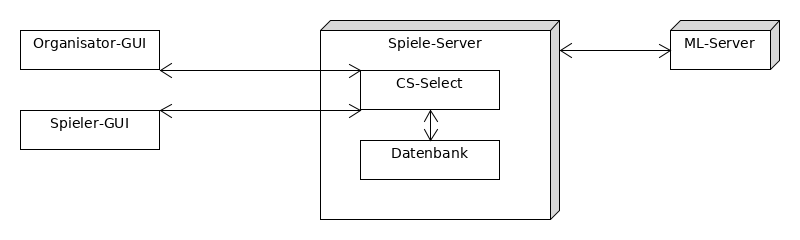
\includegraphics[width=\textwidth]{uml/export/Architektur.png}
    \section{Anwendungsbereiche}
    Das \Gls{Produkt} dient der Verbesserung der Merkmalsauswahl bei Machine-Learning Prozessen in wissenschaftlichen
    Experimenten beziehungsweise privatwirtschaftlichen Unternehmen durch das Domänenwissen der \Gls{Spieler}.

    \section{Zielgruppen}
    Die Zielgruppen des \Gls{Produkt}s lassen sich in \Glspl{Organisator} und \Glspl{Spieler} unterscheiden.
    Der Organisator möchte eine Verbesserung der Machine-Learning Prozesse erreichen, indem er das Domänenwissen der Spieler nutzt.
    Die Spieler tragen durch Spielen des \Gls{Produkt}s mit ihrem Domänenwissen zur besseren Merkmalsauswahl bei.

    \section{Betriebsbedingungen}
    Das \Gls{Produkt} ist für die Nutzung in Büroräumlichkeiten mit gewöhnlichen Arbeitsplatzrechnern vorgesehen.

    \chapter{Umgebung}
    Das \Gls{Produkt} läuft auf einem Server, die Nutzung erfolgt an Arbeitsplatzrechnern.

    \section{Software}
    Das \Gls{Produkt} läuft auf Linux ab Kernel Version 4 und Windows 7 oder neuer.
    Serverseitig benötigt das Produkt außerdem eine MYSQL-Datenbank, eine Java-Laufzeitumgebung sowie einen verfügbaren Machine-Learning-Server.
    Clientseitig wird entweder Google Chrome oder Mozilla Firefox sowie eine funktionierende Internetverbindung vorausgesetzt.

    \section{Hardware}
    Das \Gls{Produkt} läuft auf Server-Computern, das Frontend wird von gewöhnlichen Arbeitsplatzrechnern angesteuert.

    \section{Machine-Learning-Server}
    Bei dem Machine-Learning-Server handelt es sich um einen Server, der nicht Bestandteil des Produktes ist, jedoch zur Herstellung der Funktionalität benötigt wird.
    Der Machine-Learning-Server kommuniziert mit dem Produkt über das Internet mittels einer REST-API.
    Der Machine-Learning-Server übernimmt das Machine Learning und stellt die Datensätze für das Spiel zur Verfügung.
    Der Machine-Learning-Server unterstützt mindestens die nachfolgenden Anfragen:
    \begin{itemize}
        \item \texttt{GET /features} Liefert einen \Gls{Datensatz} an den Spiele-Server.
        Parameter: Datensatzidentifier
        \item \texttt{GET /score} Bewertet eine Merkmalsauswahl eines Spielers.
        Gibt eine Zahl zwischen 0 und 1 zurück, die die Güte der Merkmalsauswahl entspricht.
        Parameter: Datensatzidentifier, ausgewählte Merkmale
    \end{itemize}
    
    
    \chapter{Funktionale Anforderungen}
    
    \section{Verwaltung Spiele-Server}
    \begin{tabularx}{\linewidth}{@{}>{\bfseries}l@{\hspace{.5em}}X@{}} % Linebreaks in der Tabelle
	/F10/ & \\ 
	/F20/ & \\
	/F30/ & \\
    \end{tabularx}

    \section{Optional: Einfachere Verwaltung des Spiele-Servers}
    \begin{tabularx}{\linewidth}{@{}>{\bfseries}l@{\hspace{.5em}}X@{}} % Linebreaks in der Tabelle
	/F10/ & Bei Start des Systems gibt es ein Dialog zur Einrichtung \\ %Explizit: Was kann man da machen?
	/F20/ & Spiele aus dem System löschen \\ 
	/F30/ & Spiele-Server vom Terminal aus beenden \\
	/F40/ & Kontrollierter Neustart: Spiele-Server behält seinen Zustand über Stoppen und Starten hinweg
    \end{tabularx}
    
    \section{Nutzerverwaltung}
    \begin{tabularx}{\linewidth}{@{}>{\bfseries}l@{\hspace{.5em}}X@{}} % Linebreaks in der Tabelle
	/F10/ & Registrierung des Organisators durch global gesetztes Passwort \\ %Machen wir das so?
	/F20/ & Anmelden des Organisators \\
	/F30/ & Registrierung eines Spielers \\
	/F40/ & Anmelden eines Spielers \\
    \end{tabularx}

    \section{Optional: Zusätzliche Funktionen für Nutzerverwaltung}
    \begin{tabularx}{\linewidth}{@{}>{\bfseries}l@{\hspace{.5em}}X@{}} % Linebreaks in der Tabelle
	/F10/ & Änderung des Nutzernamens \\ %Gibt es den?
	/F20/ & Änderung des Passworts\\
	/F30/ & Zurücksetzen des Passworts ohne Kenntnis des derzeitigen Passworts \\
	/F40/ & \\
	/F50/ & \\
    \end{tabularx}
    
    \section{Spielerstellung} %ICH
    \begin{tabularx}{\linewidth}{@{}>{\bfseries}l@{\hspace{.5em}}X@{}} % Linebreaks in der Tabelle
    /F10/ & Organisator kann in Spielerstellungs-GUI Spieler zum Spiel einladen, in dem er E-Mail-Adresse angibt \\
    /F20/ & Eingeladene Spieler erhalten Einladungs-E-Mail \\
    /F30/ & Organisator muss mindestens einen Spielmodus auswählen\\
    /F40/ & Falls Matrix Select ausgewählt ist, muss Organisator Matrixgröße angeben \\
    /F50/ & Organisator muss Name des Merkmalsdatensatzes angeben \\
    /F60/ & Organisator muss Adresse einer Datenbank angeben \\ %Kann?
    /F70/ & Organisator muss Spieltitel und Spielbeschreibung angeben \\ %Kann?
    /F80/ & Organisator muss aus den folgenden mindestens eine auswählen und eventuell Werte angeben: Ende nach bestimmter Zeit, Ende nach bestimmter Anzahl an Runden, Ende durch Spielabbruch durch Organisator
    /F80/ & Organisator kann Spielerstellung abbrechen \\
    /F90/ & Organisator muss Spielerstellung bestätigen \\
    \end{tabularx}
    
    \section{Optional: Zusätzliche Funktionen bei Spielerstellung}
    \begin{tabularx}{\linewidth}{@{}>{\bfseries}l@{\hspace{.5em}}X@{}} % Linebreaks in der Tabelle
    /F10/ & Organisator kann seine Spieleinstellungen speichern \\
    /F20/ & Organisator kann seine Spieleinstellungen laden \\
    /F30/ & Organisator kann weitere Spieler nach Beginn eines Spieles einladen \\
	\end{tabularx}
    
    \section{Spielablauf} 
    \begin{tabularx}{\linewidth}{@{}>{\bfseries}l@{\hspace{.5em}}X@{}} % Linebreaks in der Tabelle
    	/F40/ & Spieler kann Einladungen zu Spielen annehmen und ablehnen \\
    	/F10/ & Spieler sieht in Spieler-Übersichts-GUI alle Spiele, bei denen er Einladung angenommen hat und die aktiv sind \\
    	/F20/ & Spieler kann Spiel auswählen und weiterspielen, anschließend: \\
    	/F30/ & Spieler spielt Runde des entsprechenden Spielmodus, für alle gilt: \\
    	/F40/ & Spieler kann Merkmal auswählen \\
    	/F40/ & Spieler kann sich zu Merkmal zusätzlich Beschreibung und Grafiken anzeigen lassen \\
    	/F40/ & Nach Beenden der Runde sieht Spieler Punktzahl und kann entscheiden, ob er noch eine Runde spielen will \\
    \end{tabularx}
    
    \subsection{Binär Select} %ICH
    \begin{tabularx}{\linewidth}{@{}>{\bfseries}l@{\hspace{.5em}}X@{}} % Linebreaks in der Tabelle
    	/F10/ & Runde Binär Select besteht aus genau fünf Vergleichen \\
    	/F20/ & Genau zwei Merkmale werden angezeigt \\
    	/F30/ & Spieler kann nur maximal eines davon auswählen \\
    	/F40/ & Spieler muss bestätigen, dafür muss er genau ein Merkmal ausgewählt haben \\
    \end{tabularx}

    \subsection{Matrix Select} %ICH
    \begin{tabularx}{\linewidth}{@{}>{\bfseries}l@{\hspace{.5em}}X@{}} % Linebreaks in der Tabelle
    	/F10/ & Runde besteht aus genau einer Matrix \\
    	/F20/ & Genau die Anzahl an Merkmalen, die Organisator bei Spielerstellung ausgewählt hat, wird angezeigt \\
    	/F30/ & Spieler kann maximal x Merkmale auswählen \\ % Wie viele Merkmale maximal? Gibt es Obergrenze?
    	/F40/ & Spieler muss bestätigen, dafür muss er genau/maximal x Merkmale ausgewählt haben \\ %Wie viele?
    \end{tabularx}
	
	\section{Optional: Zusätzliche Funktionen im Spielablauf}
	\begin{tabularx}{\linewidth}{@{}>{\bfseries}l@{\hspace{.5em}}X@{}} % Linebreaks in der Tabelle
		/F10/ & Spieler kann Runde überspringen, dann: \\
		/F20/ & Von der Gesamtpunktzahl des Spielers werden 100 Punkte abgezogen, die Gesamtpunktzahl wird aber nicht negativ \\ %100? Kann sie negativ werden?
		/F30/ & Spieler kann Merkmal als unwichtig markieren \\ 
	\end{tabularx}
	
	\section{Optional: Verbesserung der Merkmalsauswahl durch System} 
	\begin{tabularx}{\linewidth}{@{}>{\bfseries}l@{\hspace{.5em}}X@{}} % Linebreaks in der Tabelle
		/F10/ & Merkmalsauswahl durch System erfolgt nicht zufällig \\
		/F20/ & Selbe Merkmalskombination wird nicht mehrfach in einem Spiel angezeigt \\		
	\end{tabularx}
	    
    \section{Bewertung der Merkmalsauswahl des Spielers und Ergebnissicherung} %ICH
    \begin{tabularx}{\linewidth}{@{}>{\bfseries}l@{\hspace{.5em}}X@{}} % Linebreaks in der Tabelle
    /F10/ & Merkmalsauswahl des Spielers wird per http-Anfrage an ML-Server geschickt\\
    /F20/ & Bei Binär Select wird gebündelte Menge der Vergleiche geschickt \\
    /F30/ & Rückmeldung wird in Rundenpunktzahl umgewandelt \\ %Wie?
    /F40/ & Rundenpunktzahl wird zur Gesamtpunktzahl des Spielers addiert \\
    /F50/ & Rundendaten \footnote{Ausgewählte Merkmale, Spielername, Zeitpunkt, Rundenanzahl, Vorhersagequalität, Punkte} wird in von Organisator ausgewählte Datenbank gespeichert \\
    \end{tabularx}
    
    \section{GUI} %ICH
    \begin{tabularx}{\linewidth}{@{}>{\bfseries}l@{\hspace{.5em}}X@{}} % Linebreaks in der Tabelle
    /F10/ & Nutzer haben Zugriff auf die Anmeldungs-GUI in einem Webbrowser\\
    /F20/ & Organisatoren erreichen nach erfolgreicher Anmeldung die Organisator-Überschichts-GUI \\
    /F30/ & Spieler erreichen nach erfolgreicher Anmeldung die Spieler-Übersichts-GUI \\
    /F40/ & Organisatoren gelangen nach Betätigung der Spielerstellungs-Schaltfläche die Spielerstellungs-GUI \\
    /F50/ & Nach Beenden der Spielerstellung kehren Organisatoren auf die Organisator-Übersichts-GUI zurück \\
    /F60/ & Spieler gelangen nach Betätigung der "Weiterspielen"-Schaltfläche die Spiel-GUI \\
    /F70/ & Nach Beenden der Runde kehren Spieler entweder auf die Spieler-Übersichts-GUI oder die Spiel-GUI zurück \\
    /F80/ & Nach Abmeldung kehren Nutzer auf die Anmeldungs-GUI zurück \\
    \end{tabularx}
        
    \section{Gamification-Elemente}
    \begin{tabularx}{\linewidth}{@{}>{\bfseries}l@{\hspace{.5em}}X@{}} % Linebreaks in der Tabelle
    /F10/ & Punktesystem für Spieler basierend auf ihren Eingaben, erhaltener Wert des ML-Servers mit 100 multiplizieren und aufrunden    	auf nächstgrößere ganze Zahl \\
    /F20/ & \\
    \end{tabularx}

    \section{Optional: Weitere Gamification-Elemente}
    \begin{tabularx}{\linewidth}{@{}>{\bfseries}l@{\hspace{.5em}}X@{}} % Linebreaks in der Tabelle
	/F10/ & Leaderboard: Auflistung der Spieler mit den meisten Punkten %in der GUI? \\
	/F20/ & Achievements: Errungenschaften für Spieler, die freigeschaltet werden können, nachdem der Spieler bestimmte Ziele oder 		Aufgaben erledigt \\
	/F25/ & Auflistung der Achievements aus /F20/ %in der GUI?:
	/F30/ & Daily Challenges: Jeden Tag erhält ein Spieler eine neue Herausforderung, die er abschließen kann \\
	/F40/ & Streaks: Mehr Punkte für einen Spieler, wenn er zwei (oder mehrere) Spiele in Folge spielt \\
	/F50/ & Erweitertes Punktesystem: Abschließen von /F20/ und /F30/ geben zusätzliche Punkte \\
    \end{tabularx}
    
    \section{Bedienungshilfen}
	\begin{tabularx}{\linewidth}{@{}>{\bfseries}l@{\hspace{.5em}}X@{}} % Linebreaks in der Tabelle
	/F10/ & Hilfe-Schaltfläche im Organisator-GUI \\ 
	/F20/ & Hilfe Schaltfläche im Spieler-GUI \\ %Die beiden erklären?
	/F30/ &  \\
	\end{tabularx}


    \section{Internationalisierung}
    \begin{tabularx}{\linewidth}{@{}>{\bfseries}l@{\hspace{.5em}}X@{}} % Linebreaks in der Tabelle
	/F10/ & Umsetzung in der deutscher Sprache \\ 
    \end{tabularx}


    \section{Optional: Internationalisierung}
    \begin{tabularx}{\linewidth}{@{}>{\bfseries}l@{\hspace{.5em}}X@{}} % Linebreaks in der Tabelle
	/F10/ & Bereitstellung eines englischen Sprachpakets \\ 
	/F20/ & Sprachänderung \\
    \end{tabularx}

    \section{Optional: Bessere Verfügbarkeit des Systems}
    \begin{tabularx}{\linewidth}{@{}>{\bfseries}l@{\hspace{.5em}}X@{}} % Linebreaks in der Tabelle
	/F10/ & Unterstützung von Internet Explorer \\
	/F20/ & Unterstützung von Mobilgeräten mit Responsive-GUIs \\
	/F30/ & Lieferung des Servers als Docker-Image \\
	/F40/ & Der Server kann auf verschiedenen Ports ausgeführt werden \\
    \end{tabularx}

    \chapter{Produktdaten}

    \section{Nutzerdaten}
    \begin{tabularx}{\linewidth}{@{}>{\bfseries}l@{\hspace{.5em}}X@{}}
        /D10/ & Über Nutzer(\Gls{Spieler}, \Gls{Organisator}) sind folgende Daten zu speichern /ND10/: 
        \begin{itemize}
              \item Email-Adresse, Nutzername, Punktestand, Rolle, Passwort(als Hash)
        \end{itemize} \\
        /KD10/ & Über einen \Gls{Spieler} werden außerdem seine Achievements gespeichert. \\
        /KD20/ & Über einen \Gls{Organisator} werden außerdem seine Spieleinstellungen gespeichert. \\
    \end{tabularx}

    \section{Merkmalsdatensätze}
    \begin{tabularx}{\linewidth}{@{}>{\bfseries}l@{\hspace{.5em}}X@{}}
        /D20/ & Für jeden Merkmalsdatensatz ist zu speichern: /ND20/: 
        \begin{itemize}
             \item Liste an Merkmalen mit jeweiligen Graphen und Beschreibung
        \end{itemize}
    \end{tabularx}

    \section{Spieledaten}
    \begin{tabularx}{\linewidth}{@{}>{\bfseries}l@{\hspace{.5em}}X@{}}
        /D30/ & Für jedes \Gls{Spiel} ist zu speichern /ND30/: 
        \begin{itemize}
             \item \Gls{Organisator}, \Gls{Spieleinstellungen}, \Gls{Spieler}, zugehöriger Merkmalsdatensatz % zuständiger ML Server?
        \end{itemize}
    \end{tabularx}


    \chapter{Nichtfunktionale Anforderungen}

    \begin{tabular}{ l l}
        /NF10/ & Es müssen mindestens 30 Spieler zur gleichen Zeit spielen können.\\
        /NF20/ & Die Interaktionszeiten dürfen nicht länger als zwei Sekunden betragen. \\
        /NF30/ & Ein Spieler soll das Ergebnis seines Spiels innerhalb von zwei Sekunden erhalten. \\
        /NF40/ & Das Design soll modern sein. \\
        /NF50/ & Der \Gls{ML-Server} soll leicht austauschbar sein. \\
        /NF60/ & Neue Spielmodi sollen leicht hinzugefügt werden können. \\
        /NF70/ & Neue Spieloberflächen sollen leicht erweiterbar sein. \\
        /NF80/ & Neue Sprachen sollen leicht hinzugefügt werden können. \\
        /NF90/ & Das Produkt enthält nicht mehr als 0,1\% plattformspezifischer Anweisungen. \\
        /NF100/ & Es gibt nicht mehr als einen Ausfall des Systems pro Monat. \\ %Realistisch?
        /NF110/ & Die Anmeldedauer darf nicht mehr als zwei Sekunden betragen. \\
        /NF120/ & Die Daten zu den Spielergebnissen werden strukturiert und menschenlesbar abgespeichert.\footnotemark\\
    \end{tabular}
    \footnotetext{Also .csv oder eine Datenbank} 

    \chapter{Systemmodelle}
    \section{Anwendungsfälle}

    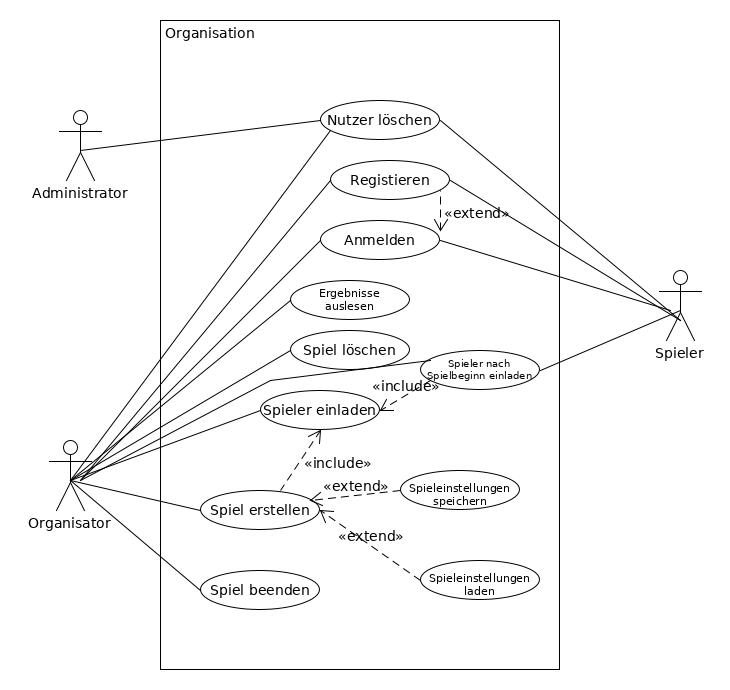
\includegraphics[width=\textwidth]{uml/export/Organisation.png}
    Akteure:
    \begin{itemize}
        \item \Gls{Administrator}
        \item \Gls{Organisator}
        \item \Gls{Spieler}
    \end{itemize}
    \newpage
   \subsection{Spieler registrieren}
    \begin{itemize}
        \item Teilnehmende Akteure: \Gls{Organisator}, \Gls{Spieler}
        \item Eingangsaktionen: Spiele-Server ist aktiv
        \item Ereignisfluss:
        \begin{itemize}
            \item Organisator lädt den Spieler über das Organisator-GUI ein.
            \item Der Spieler klickt auf den Einladungslink in der E-Mail und wird auf die Registrierungsseite weitergeleitet.
            \item Der Spieler gibt einen einzigartigen Nutzernamen, seine E-Mail-Adresse sowie ein persönliches Passwort ein und bestätigt.
        \end{itemize}
    \end{itemize}

    \subsection{Spieler anmelden}
    \begin{itemize}
        \item Teilnehmende Akteure: \Gls{Spieler}
        \item Eingangsaktionen: Spiele-Server ist aktiv
        \item Ereignisfluss:
        \begin{itemize}
            \item Spieler öffnet die Produktwebsite
            \item Spieler wählt die Rolle "Spieler" aus
            \item Spieler gibt E-Mail und Passwort ein
            \item Spieler klickt auf anmelden
        \end{itemize}
    \end{itemize}

    \subsection{Spieler löschen}
    \begin{itemize}
        \item Teilnehmende Akteure: \Gls{Administrator}
        \item Eingangsaktionen: Spiele-Server ist aktiv
        \item Ereignisfluss:
        \begin{itemize}
            \item Administrator loggt sich am Server ein
            \item Administrator führt das Löschen-Kommando mit dem Nutzernamen des zu löschenden Spielers aus
            \item Administrator bestätigt den Vorgang
        \end{itemize}
    \end{itemize}

    \subsection{Organisator registrieren}
    \begin{itemize}
        \item Teilnehmende Akteure: \Gls{Organisator}
        \item Eingangsaktionen: Spiele-Server ist aktiv, Organisator-Registrierungspasswort ist gesetzt
        \item Ereignisfluss:
        \begin{itemize}
            \item Organisator öffnet die Produktwebsite und klickt auf Registrieren
            \item Organisator gibt einen einzigartigen Nutzernamen, seine E-Mail-Adresse, das Organisator-Registrierungspasswort sowie ein persönliches Passwort ein und bestätigt seine Auswahl
        \end{itemize}
    \end{itemize}

    \subsection{Organisator anmelden}
    \begin{itemize}
        \item Teilnehmende Akteure: \Gls{Organisator}
        \item Eingangsaktionen: Spiele-Server ist aktiv
        \item Ereignisfluss:
        \begin{itemize}
            \item Organisator öffnet die Produktwebsite
            \item Organisator wählt die Rolle "Organisator" aus
            \item Organisator gibt E-Mail und Passwort ein
            \item Organisator klickt auf anmelden
        \end{itemize}
    \end{itemize}

    \subsection{Organisator löschen}
    \begin{itemize}
        \item Teilnehmende Akteure: \Gls{Administrator}
        \item Eingangsaktionen: Spiele-Server ist aktiv
        \item Ereignisfluss:
        \begin{itemize}
            \item Administrator loggt sich am Server ein
            \item Administrator führt das Löschen-Kommando mit dem Nutzernamen des zu löschenden Organisators aus
            \item Administrator bestätigt den Vorgang
        \end{itemize}
    \end{itemize}

    \subsection{Spiel erstellen}
    \begin{itemize}
        \item Teilnehmende Akteure: \Gls{Organisator}, \Gls{Spieler}
        \item Eingangsaktionen: Spiele-Server ist aktiv
        \item Ausgangsaktionen: Spiel starten, Spieler werden eingeladen
        \item Ereignisfluss:
        \begin{itemize}
            \item Organisator meldet sich an
            \item Organisator klickt auf "Spiel erstellen"-Schaltfläche
            \item Organisator sucht sich über seine GUI die gewünschten Spieleinstellungen aus
            \item Organisator lädt Spieler über Angabe der Email in einem Textfeld ein
            \item Organisator bestätigt seine Auswahl und erstellt das Spiel
        \end{itemize}
    \end{itemize}

    \subsection{Spieler nach Spielbeginn einladen}
    \begin{itemize}
        \item Teilnehmende Akteure: \Gls{Organisator}, \Gls{Spieler}
        \item Eingangsaktionen: Spiele-Server ist aktiv, Spiel ist gestartet
        \item Ausgangsaktionen: Spieler werden eingeladen
        \item Ereignisfluss:
        \begin{itemize}
            \item Organisator meldet sich an
            \item Organisator wählt gestartetes Spiel aus der Übersicht
            \item Organisator betätigt "Einladen"-Schaltfläche
            \item Organisator tippt Emails der Spieler in Textfeld ein
            \item Organisator bestätigt seine Auswahl
        \end{itemize}
    \end{itemize}

    \subsection{Spiel vorzeitig beenden}
    \begin{itemize}
        \item Teilnehmende Akteure: \Gls{Organisator}, \Gls{Spieler}
        \item Eingangsaktionen: Spiel ist aktiv und gestartet
        \item Ausgangsaktionen: Spieler können Spiel nicht mehr spielen %werden sie benachrichtigt?
        \item Ereignisfluss:
        \begin{itemize}
            \item Organisator meldet sich an
            \item Organisator wählt gestartetes Spiel aus der Übersicht
            \item Organisator betätigt "Beenden"-Schaltfläche
            \item Organisator bestätigt seine Auswahl
        \end{itemize}
    \end{itemize}

    \subsection{Spiel löschen}
    \begin{itemize}
        \item Teilnehmende Akteure: \Gls{Organisator}
        \item Eingangsaktionen: Spiele-Server ist aktiv, es existiert bereits ein Spiel
        \item Ausgangsaktionen: Spiel löschen
        \item Ereignisfluss:
        \begin{itemize}
            \item Organisator meldet sich an
            \item Organisator wählt über seine GUI das zu löschende Spiel
            \item Organisator bestätigt seine Auswahl
        \end{itemize}
    \end{itemize}

    \subsection{Spieleinstellungen speichern}
    \begin{itemize}
        \item Teilnehmende Akteure: \Gls{Organisator}
        \item Eingangsaktionen: Spiele-Server ist aktiv
        \item Ausgangsaktionen: Spieleinstellungen wiederverwenden
        \item Ereignisfluss:
        \begin{itemize}
            \item Organisator meldet sich an
            \item Organisator sucht sich über seine GUI das Spiel aus, von dem er die Einstellungen speichern möchte
            \item Organisator wählt die Option \enquote{Spieleinstellungen speichern}
            \item Organisator bestätigt seine Auswahl und speichert die Einstellungen
        \end{itemize}
    \end{itemize}

    \subsection{Spieleinstellungen laden}
    \begin{itemize}
        \item Teilnehmende Akteure: \Gls{Organisator}
        \item Eingangsaktionen: Spiele-Server ist aktiv, Spieleinstellungen wurden bereits gespeichert
        \item Ausgangsaktionen: Spiel starten
        \item Ereignisfluss:
        \begin{itemize}
            \item Organisator meldet sich an
            \item Organisator erstellt über seine GUI ein neues Spiel
            \item Organisator wählt für dieses Spiel \enquote{Spieleinstellungen laden}
            \item Organisator sucht sich die bereits gespeicherte Spieleinstellungen heraus
            \item Organisator bestätigt seine Auswahl
        \end{itemize}
    \end{itemize}

    \subsection{Ergebnisse auslesen}

    \begin{itemize}
        \item Teilnehmende Akteure: \Gls{Organisator}
        \item Eingangsaktionen: \Gls{Organisator} öffnet die Auswertungsseite
        \item Ausgangsaktionen: \Gls{Organisator} erhält die Auswertung
        \item Ereignisfluss -
    \end{itemize}
 \subsection{Spielzustand auslesen}
	\begin{itemize}
		\item Teilnehmende Akteure: \Gls{Organisator}
		\item Eingangsaktionen: Spiele-Server ist aktiv
		\item Ereignisfluss:
		\begin{itemize}
			\item Organisator meldet sich an
			\item Organisator erreicht seine Übersichtsseite
			\item Organisator sieht den Zustand seiner laufenden Spiele
		\end{itemize}
	\end{itemize}


    \newpage
    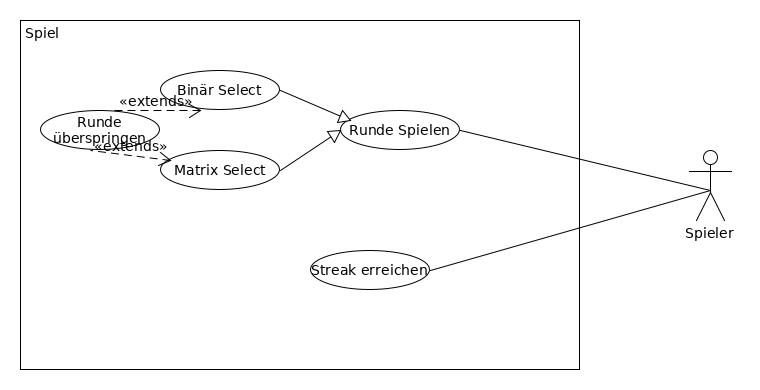
\includegraphics[width=\textwidth]{uml/export/Spiel.png}
    Akteure: 
    \begin{itemize}
    \item \Gls{Spieler}
    \newpage
    \end{itemize}
    
   
    \subsection{Runde spielen: Matrix Select}
    \begin{itemize}
    	\item Teilnehmende Akteure: \Gls{Spieler}
    	\item Eingangsaktionen: Spiele-Server ist aktiv, Spieler hat offenes Spiel des Spielmodus Matrix Select
    	\item Ereignisfluss:
    	\begin{itemize}
    		\item Spieler meldet sich an
    		\item Spieler erreicht seine Übersichtsseite
    		\item Spieler klickt auf Weiterspielen-Schaltfläche
    		\item Spieler erreicht Spiel-GUI
    		\item Spieler klickt auf ein Merkmal und sieht Merkmalsgraphen und Merkmalsbeschreibung
    		\item Spieler wählt mehrere Merkmale aus
    		\item Spieler klickt auf Schaltfläche, um Auswahl zu bestätigen 
    	\end{itemize}
    \end{itemize}
	
	\subsection{Runde spielen: Binär Select}
	\begin{itemize}
		\item Teilnehmende Akteure: \Gls{Spieler}
		\item Eingangsaktionen: Spiele-Server ist aktiv, Spieler hat offenes Spiel des Spielmodus Binär Select
		\item Ereignisfluss:
		\begin{itemize}
			\item Spieler meldet sich an
			\item Spieler erreicht seine Übersichtsseite
			\item Spieler klickt auf Weiterspielen-Schaltfläche
			\item Spieler erreicht Spiel-GUI
			\item Spieler klickt auf ein Merkmal und sieht Merkmalsgraphen und Merkmalsbeschreibung
			\item Spieler wählt eines der beiden Merkmale aus
			\item Spieler klickt auf Schaltfläche, um Auswahl zu bestätigen 
		\end{itemize}
	\end{itemize}

	\subsection{Auswahl überspringen}
	\begin{itemize}
		\item Teilnehmende Akteure: \Gls{Spieler}
		\item Eingangsaktionen: Spiele-Server ist aktiv, Spieler hat offenes Spiel
        \item Ausgangsaktionen: Der Spieler kommt in die nächste Runde des aktiven Spiels
		\item Ereignisfluss:
		\begin{itemize}
			\item Spieler meldet sich an
			\item Spieler erreicht seine Übersichtsseite
			\item Spieler klickt auf Weiterspielen-Schaltfläche
			\item Spieler erreicht Spiel-GUI
			\item Spieler klickt Auswahl-Überspringen-Schaltfläche und bestätigt seine Auswahl
            \item Dem Spieler werden Punkte abgezogen
		\end{itemize}
	\end{itemize}
     
    \subsection{Streak erreichen}\footnote{Zur Erklärung von Streak siehe \fref{fig:Streak_State}}
    \begin{itemize}
        \item Teilnehmende Akteure: \Gls{Spieler}
        \item Eingangsaktionen: Spieler spielt eine Runde
        \item Ausgangsaktionen: Spieler erhält extra Punkte für seine Runde
        \item Ereignisfluss:
        \begin{itemize}
            \item Spieler spielt n Runden um eine Streak zu erreichen. 
            \item System teilt dem Spieler mit, dass er eine Streak erreicht hat.
        \end{itemize}
    \end{itemize}
    
\newpage
    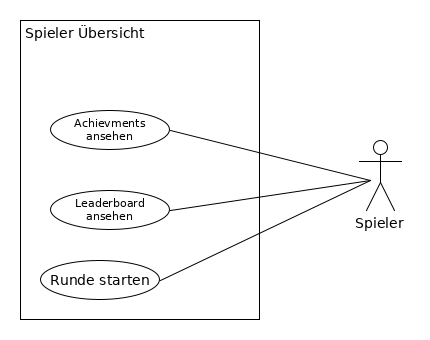
\includegraphics[width=\textwidth]{uml/export/Spieler_Ubersicht.png}
	    \subsection{Achievements ansehen}
    \begin{itemize}
        \item Teilnehmende Akteure: \Gls{Spieler}
        \item Eingangsaktionen: Spiele-Server ist aktiv
        %\item Ausgangsaktionen: Achievements ansehen
        \item Ereignisfluss:
        \begin{itemize}
            \item Spieler meldet sich an
            \item Spieler erreicht seine Übersicht-Seite
            \item Spieler klickt auf die Spieler-Übersicht-Schaltfläche
            \item Spieler schaut seine Achievements an
        \end{itemize}
    \end{itemize}
    %Nach der Anmeldung erreicht ein \Gls{Spieler} eine Übersichts-Seite. Beim Klicken auf die Spieler-Übersicht-Schaltfläche
    %(in \fref{fig:Spieler-Übersicht} gezeigt) kann der \Gls{Spieler} seine \Gls{Achievement}s einsehen.
    \subsection{Leaderboard ansehen}
    \begin{itemize}
        \item Teilnehmende Akteure: \Gls{Spieler}
        \item Eingangsaktionen: Spiele-Server ist aktiv
        %\item Ausgangsaktionen: Leaderboard ansehen
        \item Ereignisfluss:
        \begin{itemize}
            \item Spieler meldet sich an
            \item Spieler erreicht seine Übersichtsseite
            \item Spieler sieht dort in einer Tabelle die Spieler mit den meisten Punkten über einen gewissen Zeitraum
        \end{itemize}
    \end{itemize}
    %Nach der Anmeldung erreicht ein \Gls{Spieler} eine Übersichts-Seite. Darauf ist ein Bereich, der eine aktuelle Tabelle
    %anzeigt, in welcher die \Gls{Spieler} aufgelistet sind, die in einem bestimmten Zeitraum die meisten Punkte erreicht haben.
    \newpage
    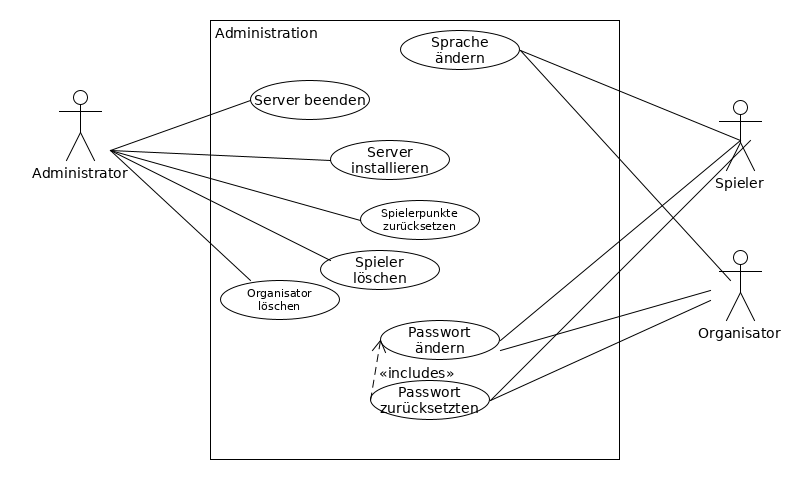
\includegraphics[width=\textwidth]{uml/export/Administration.png}
     \subsection{Sprache ändern}
    \begin{itemize}
    \item Teilnehmende Akteure: \Gls{Spieler}, \Gls{Organisator}
    \item Eingangsaktionen: Spiele-Server ist aktiv
    \item Ereignisfluss:
        \begin{itemize}
            \item Organisator oder Spieler meldet sich an
            \item Organisator oder Spieler erreicht seine Übersichtsseite
            \item Organisator oder Spieler wählt die Sprachänderungs-Schaltfläche aus
            \item Organisator oder Spieler bestätigt seine Auswahl
        \end{itemize}
    \end{itemize}
    \subsection{Server installieren}
    \begin{itemize}
        \item Teilnehmende Akteure: \Gls{Administrator} 
        \item Eingangsaktionen: Computer mit MySQL und Tomcat installiert
        \item Ausgangsaktionen: Spiele-Server starten
        \item Ereignisfluss: 
            \begin{itemize}
                \item Administrator kopiert die War Datei in den Tomcat webapps Ordner
                \item Administrator fügt den Pfad zur CFG Datei in die `tomcat/conf/Catalina/<host>` Datei ein
                \item Administrator konfiguriert die CFG Datei aus der Dokumentation mit den relevanten Werten
                \item Administrator führt \texttt{tomcat/bin/startup.sh}(Linux \& Mac) bzw. \texttt{tomcat\textbackslash bin\textbackslash startup.bat}(Windows) aus
            \end{itemize}
    \end{itemize}

    \subsection{Server beenden}
    \begin{itemize}
        \item Teilnehmende Akteure: \Gls{Administrator}
        \item Eingangsaktionen: Spiele-Server ist aktiv
        \item Ausgangsaktionen: MySQL beenden, falls sonst nichts Weiteres auf der Datenbank läuft
        \item Ereignisfluss: Administrator führt \texttt{tomcat/bin/shutdown.sh}(Linux \& Mac) bzw. \texttt{tomcat\textbackslash bin\textbackslash shutdown.bat}(Windows)
    \end{itemize}

    \subsection{Punkte eines Spielers zurücksetzen}
    \begin{itemize}
        \item Teilnehmende Akteure: \Gls{Administrator}, \Gls{Spieler}
        \item Eingangsaktionen: Spiele-Server ist aktiv
        \item Ausgangsaktionen: Die Punkte des Spielers sind zurückgesetzt
        \item Ereignisfluss:
        \begin{itemize}
            \item Administrator loggt sich in Spiele-Server ein
            \item Administrator gibt das "Punkte zurücksetzen"-Kommando und die Email des registrierten Spielers ein
            \item Administrator bestätigt seine Auswahl
            \item Die Punkte des entsprechenden Spielers werden zurückgesetzt
        \end{itemize}
    \end{itemize}




    \subsection{Passwort ändern}
    \begin{itemize}
    \item Teilnehmende Akteure: \Gls{Spieler}, \Gls{Organisator}
    \item Eingangsaktionen: Spiele-Server ist aktiv
    \item Ereignisfluss:
        \begin{itemize}
            \item Organisator oder Spieler meldet sich an
            \item Organisator oder Spieler erreicht seine Übersichtsseite
            \item Organisator oder Spieler wählt die Profileinstellungen aus
            \item Organisator oder Spieler klickt aus die \enquote{Passwort ändern}-Schaltfläche
            \item Organisator oder Spieler gibt sein aktuelle sowie sein neues gewünschtes Passwort ein
            \item Organisator oder Spieler bestätigt seine Auswahl
        \end{itemize}
    \end{itemize}

    \subsection{Passwort zurücksetzen}
    \begin{itemize}
        \item Teilnehmende Akteure: \Gls{Spieler}, \Gls{Organisator}
        \item Eingangsaktionen: Spiele-Server ist aktiv
        \item Ausgangsaktionen: Temporäres Passwort ändern
        \item Ereignisfluss:
        \begin{itemize}
            \item Organisator oder Spieler öffnet die Produktwebsite und klickt auf \enquote{Passwort zurücksetzen}
            \item Organisator oder Spieler erhält per Mail ein neues temporäres Passwort
            \item Organisator oder Spieler meldet sich mit dem neuen Passwort an
        \end{itemize}
    \end{itemize}
       \subsection{Hilfe-Schaltfläche verwenden}
    \begin{itemize}
        \item Teilnehmende Akteure: \Gls{Spieler}, \Gls{Organisator}
        \item Eingangsaktionen: Spieler oder Organisator benötigt Hilfe mit dem Produkt
        \item Ausgangsaktionen: System zeigt dem Akteur die relevante Hilfe Seite
        \item Ereignisfluss:
            \begin{itemize}
                \item Spieler oder Organisator klickt auf die Hilfe-Schaltfläche(oben links)
            \end{itemize}
    \end{itemize}

    %TODO: Ausführung auf verschiedenem Ports

        \section{Objektmodell}

    \section{Dynamische Modelle}
    \subsection{Streak Zustandsdiagramm}
    \label{fig:Streak_State}
    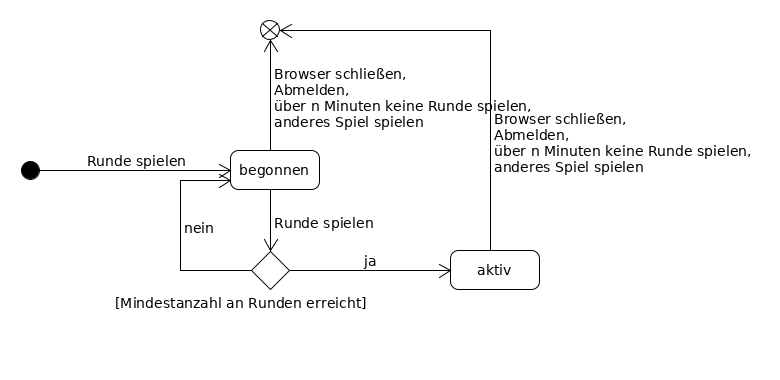
\includegraphics[width=\textwidth]{uml/export/Streak_Zustand.png}
    \subsection{Spiel Zustandsdiagramm}
    \label{fig:Spiel_State}
    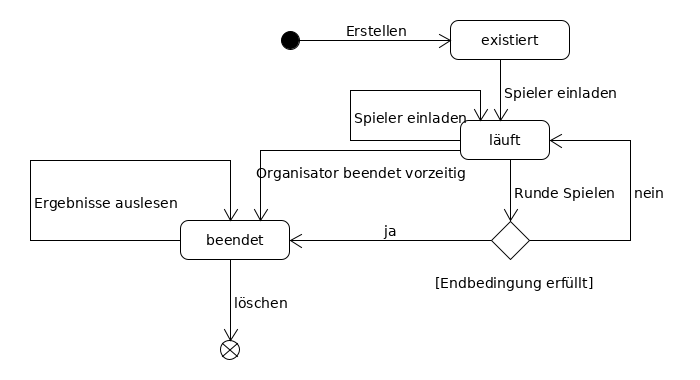
\includegraphics[width=\textwidth]{uml/export/Spiel_Zustand.png}
    \subsection{Achievements Zustandsdiagramm}
    \label{fig:Achievment_State}
    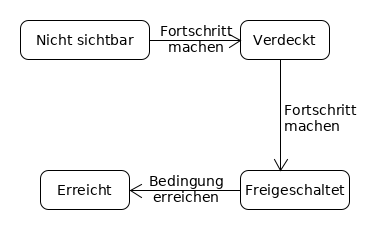
\includegraphics[width=\textwidth]{uml/export/Achievment_State.png}
    

    \chapter{Benutzerschnittstelle}

    \section{Anmeldung}
    \centering
    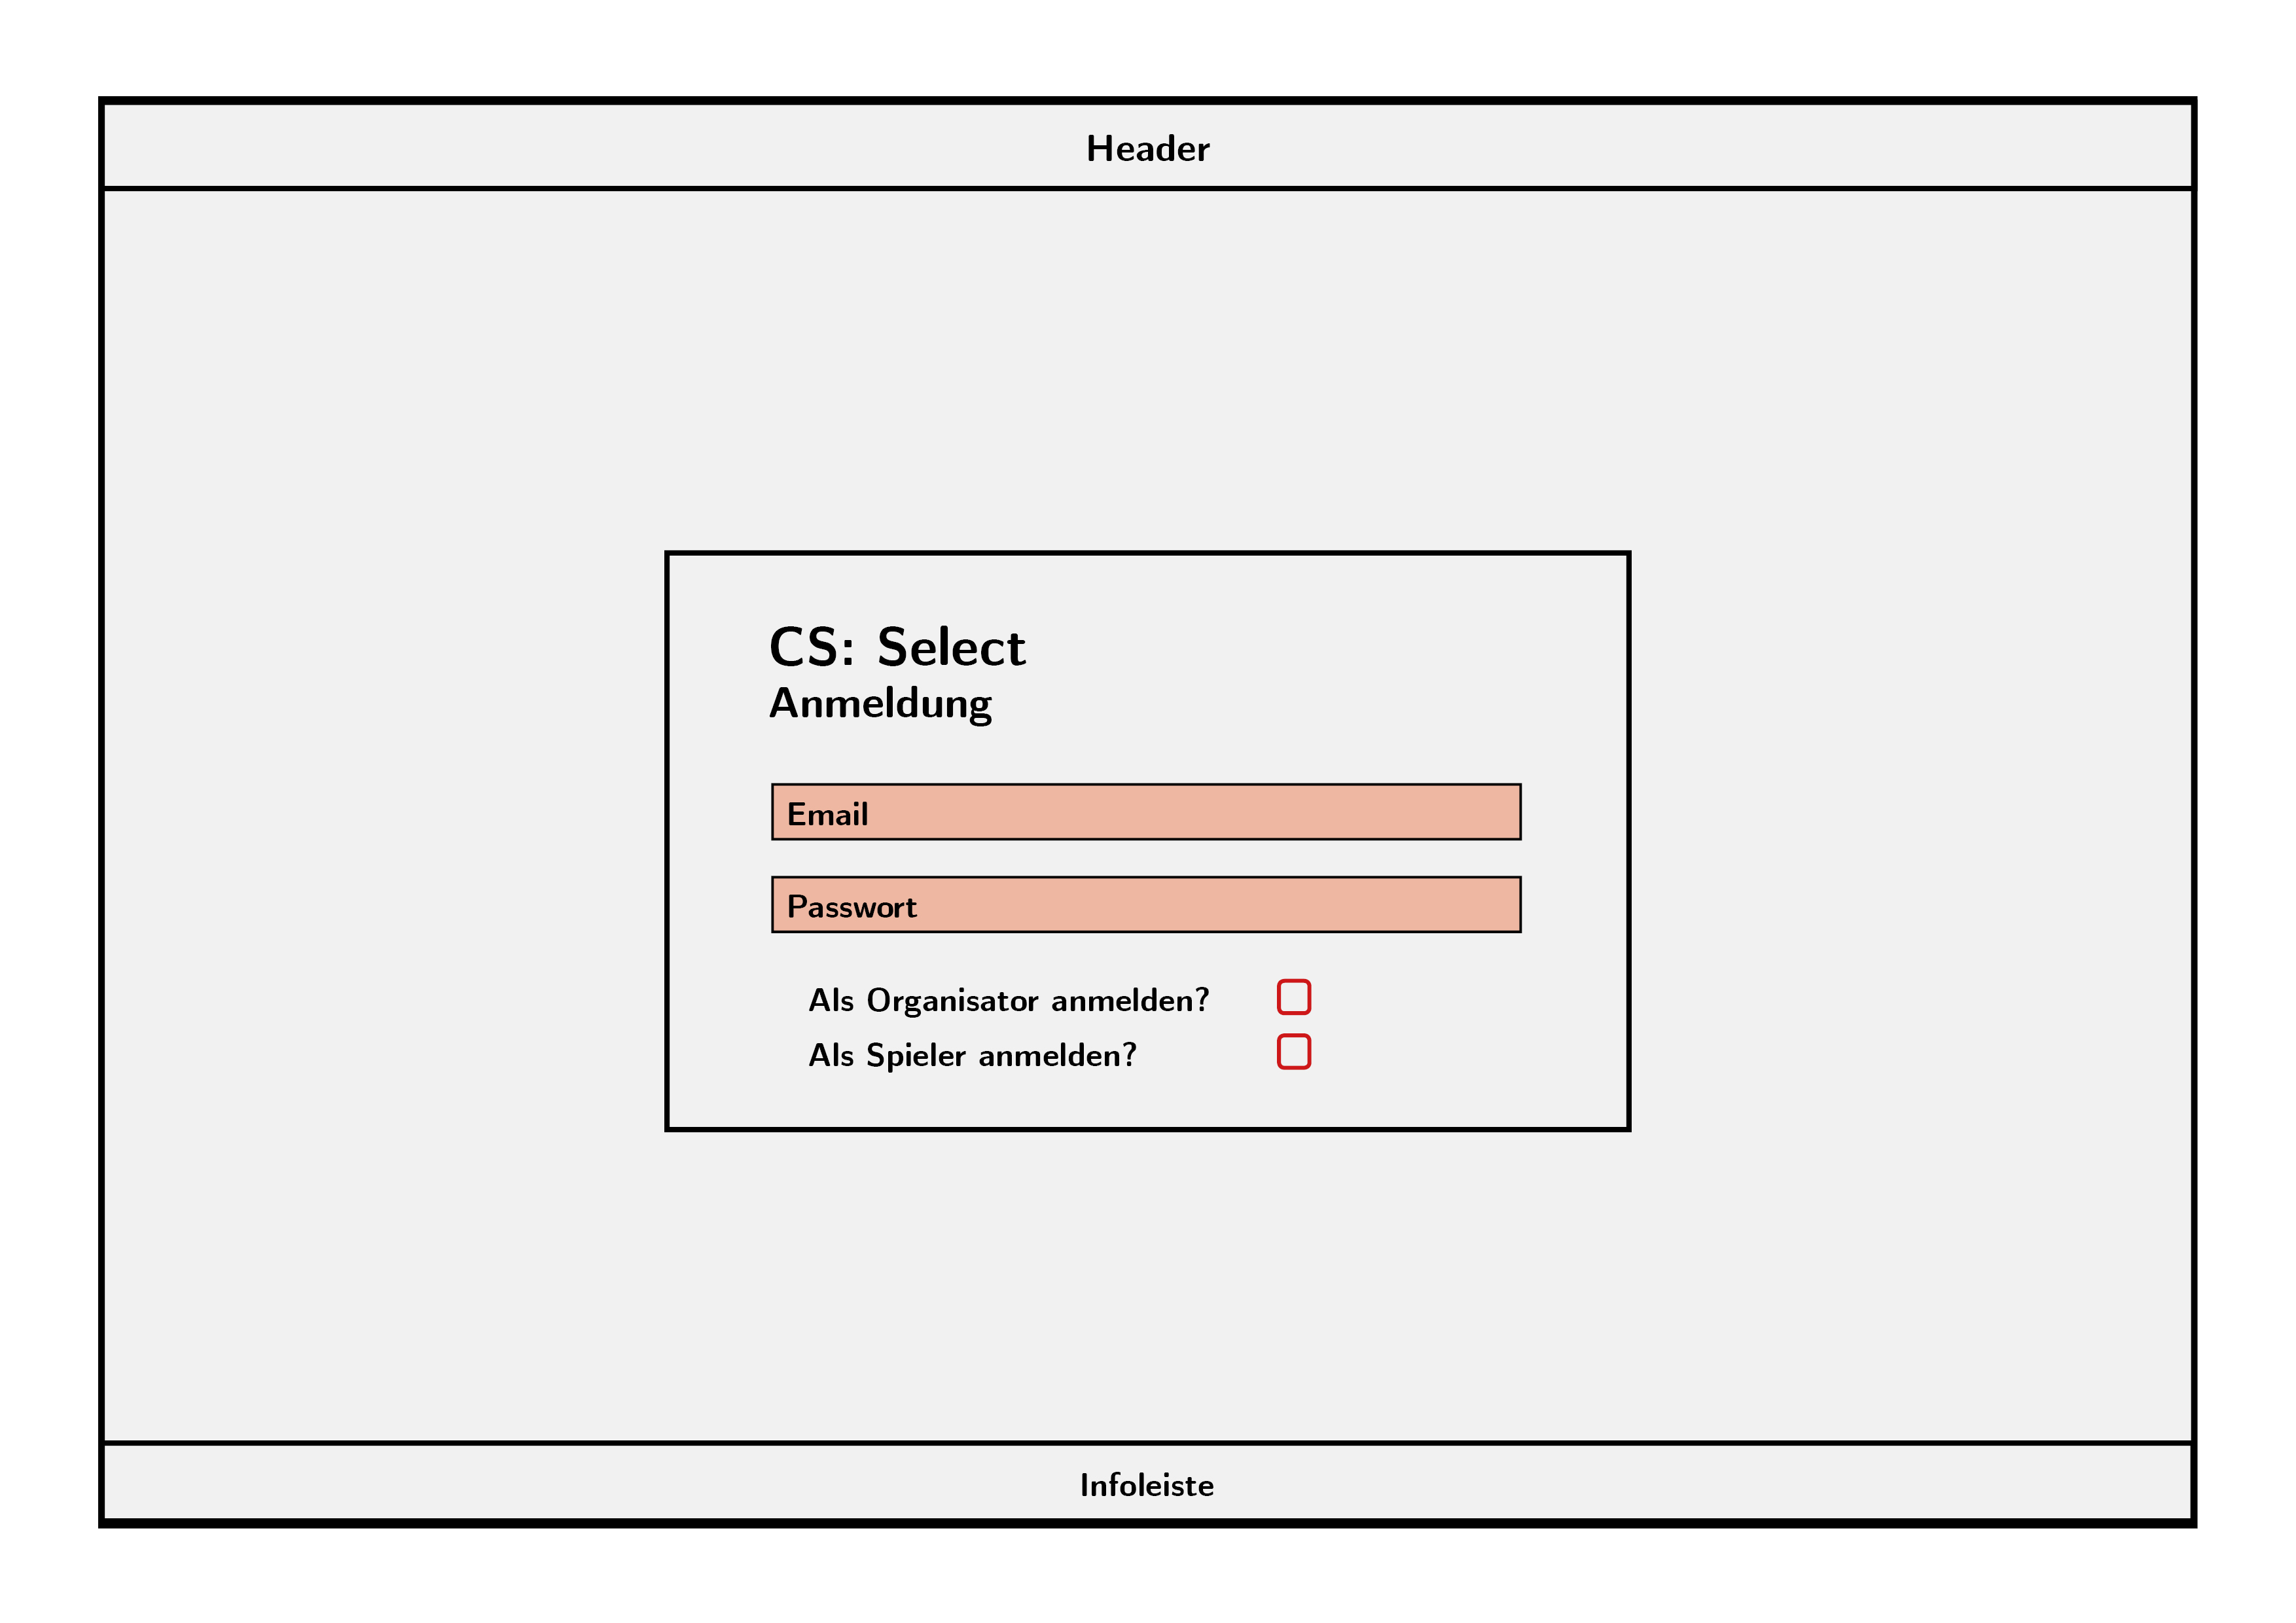
\includegraphics[width=\textwidth]{../pictures/Anmeldung.jpg}
    \subsection{Anmeldung (responsive)}
    \centering
    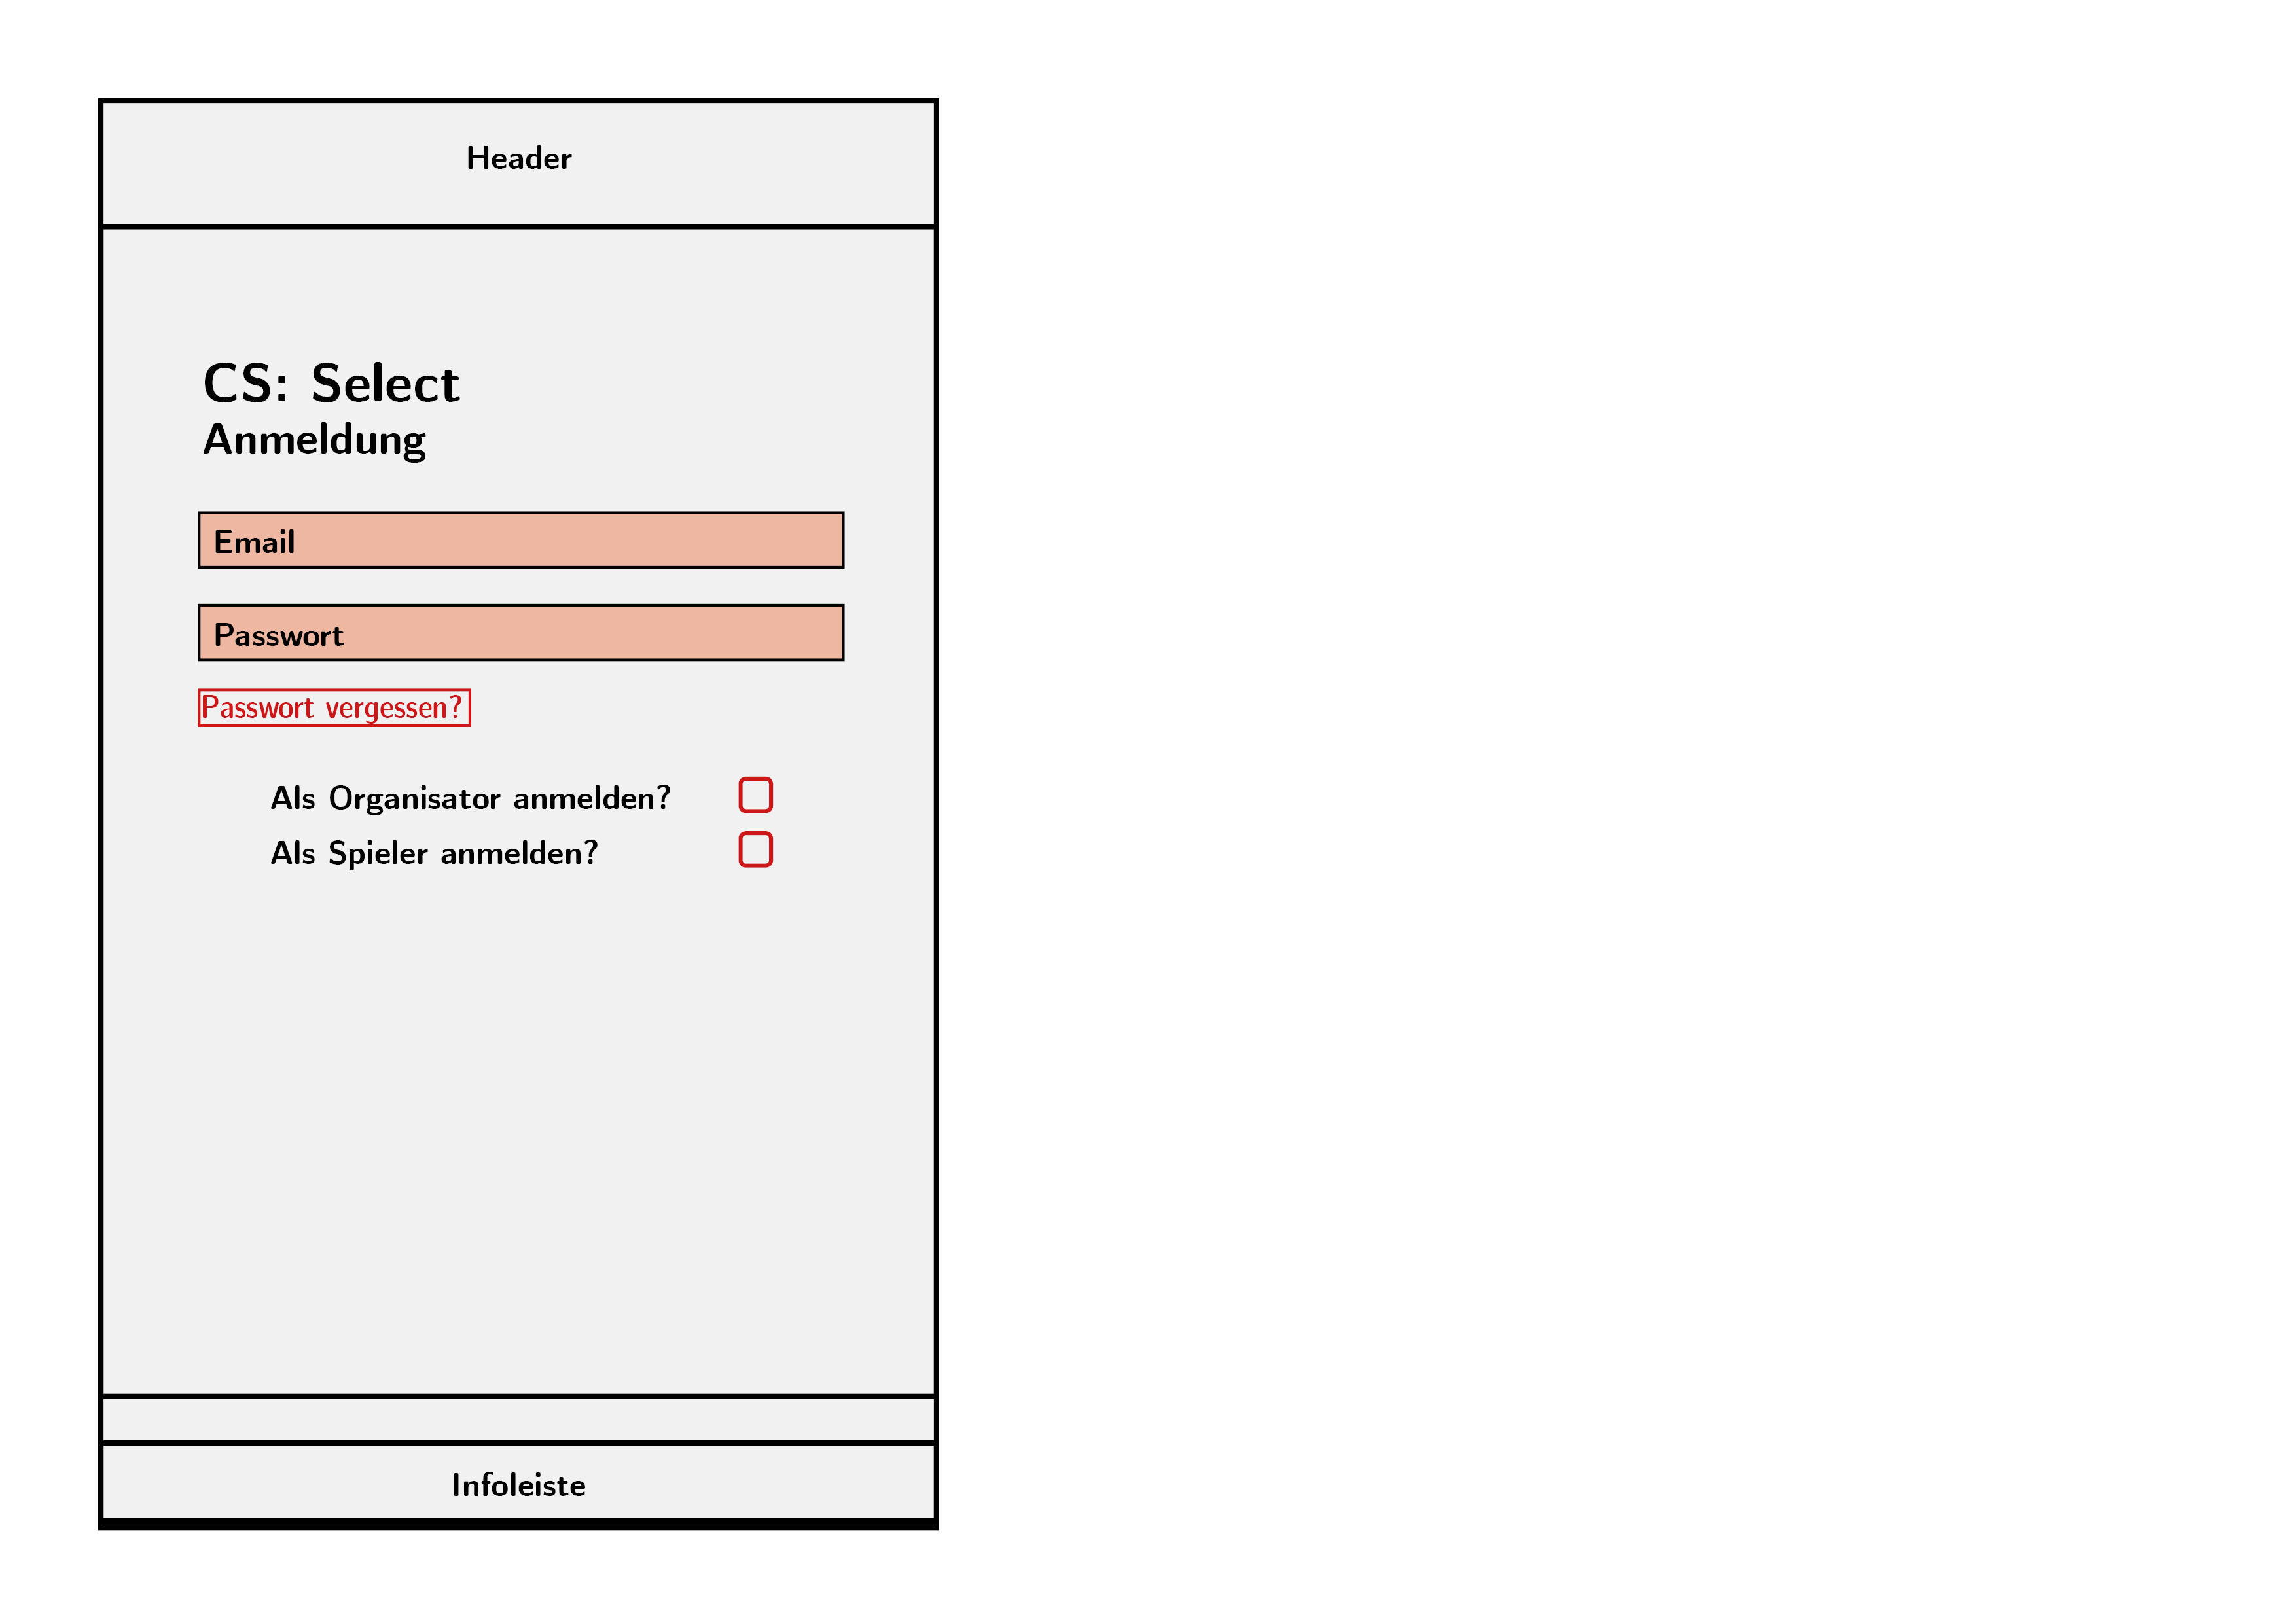
\includegraphics[width=\textwidth]{../pictures/Anmeldung_responsive.jpg}

    \section{Organisator-Start}
    \centering
    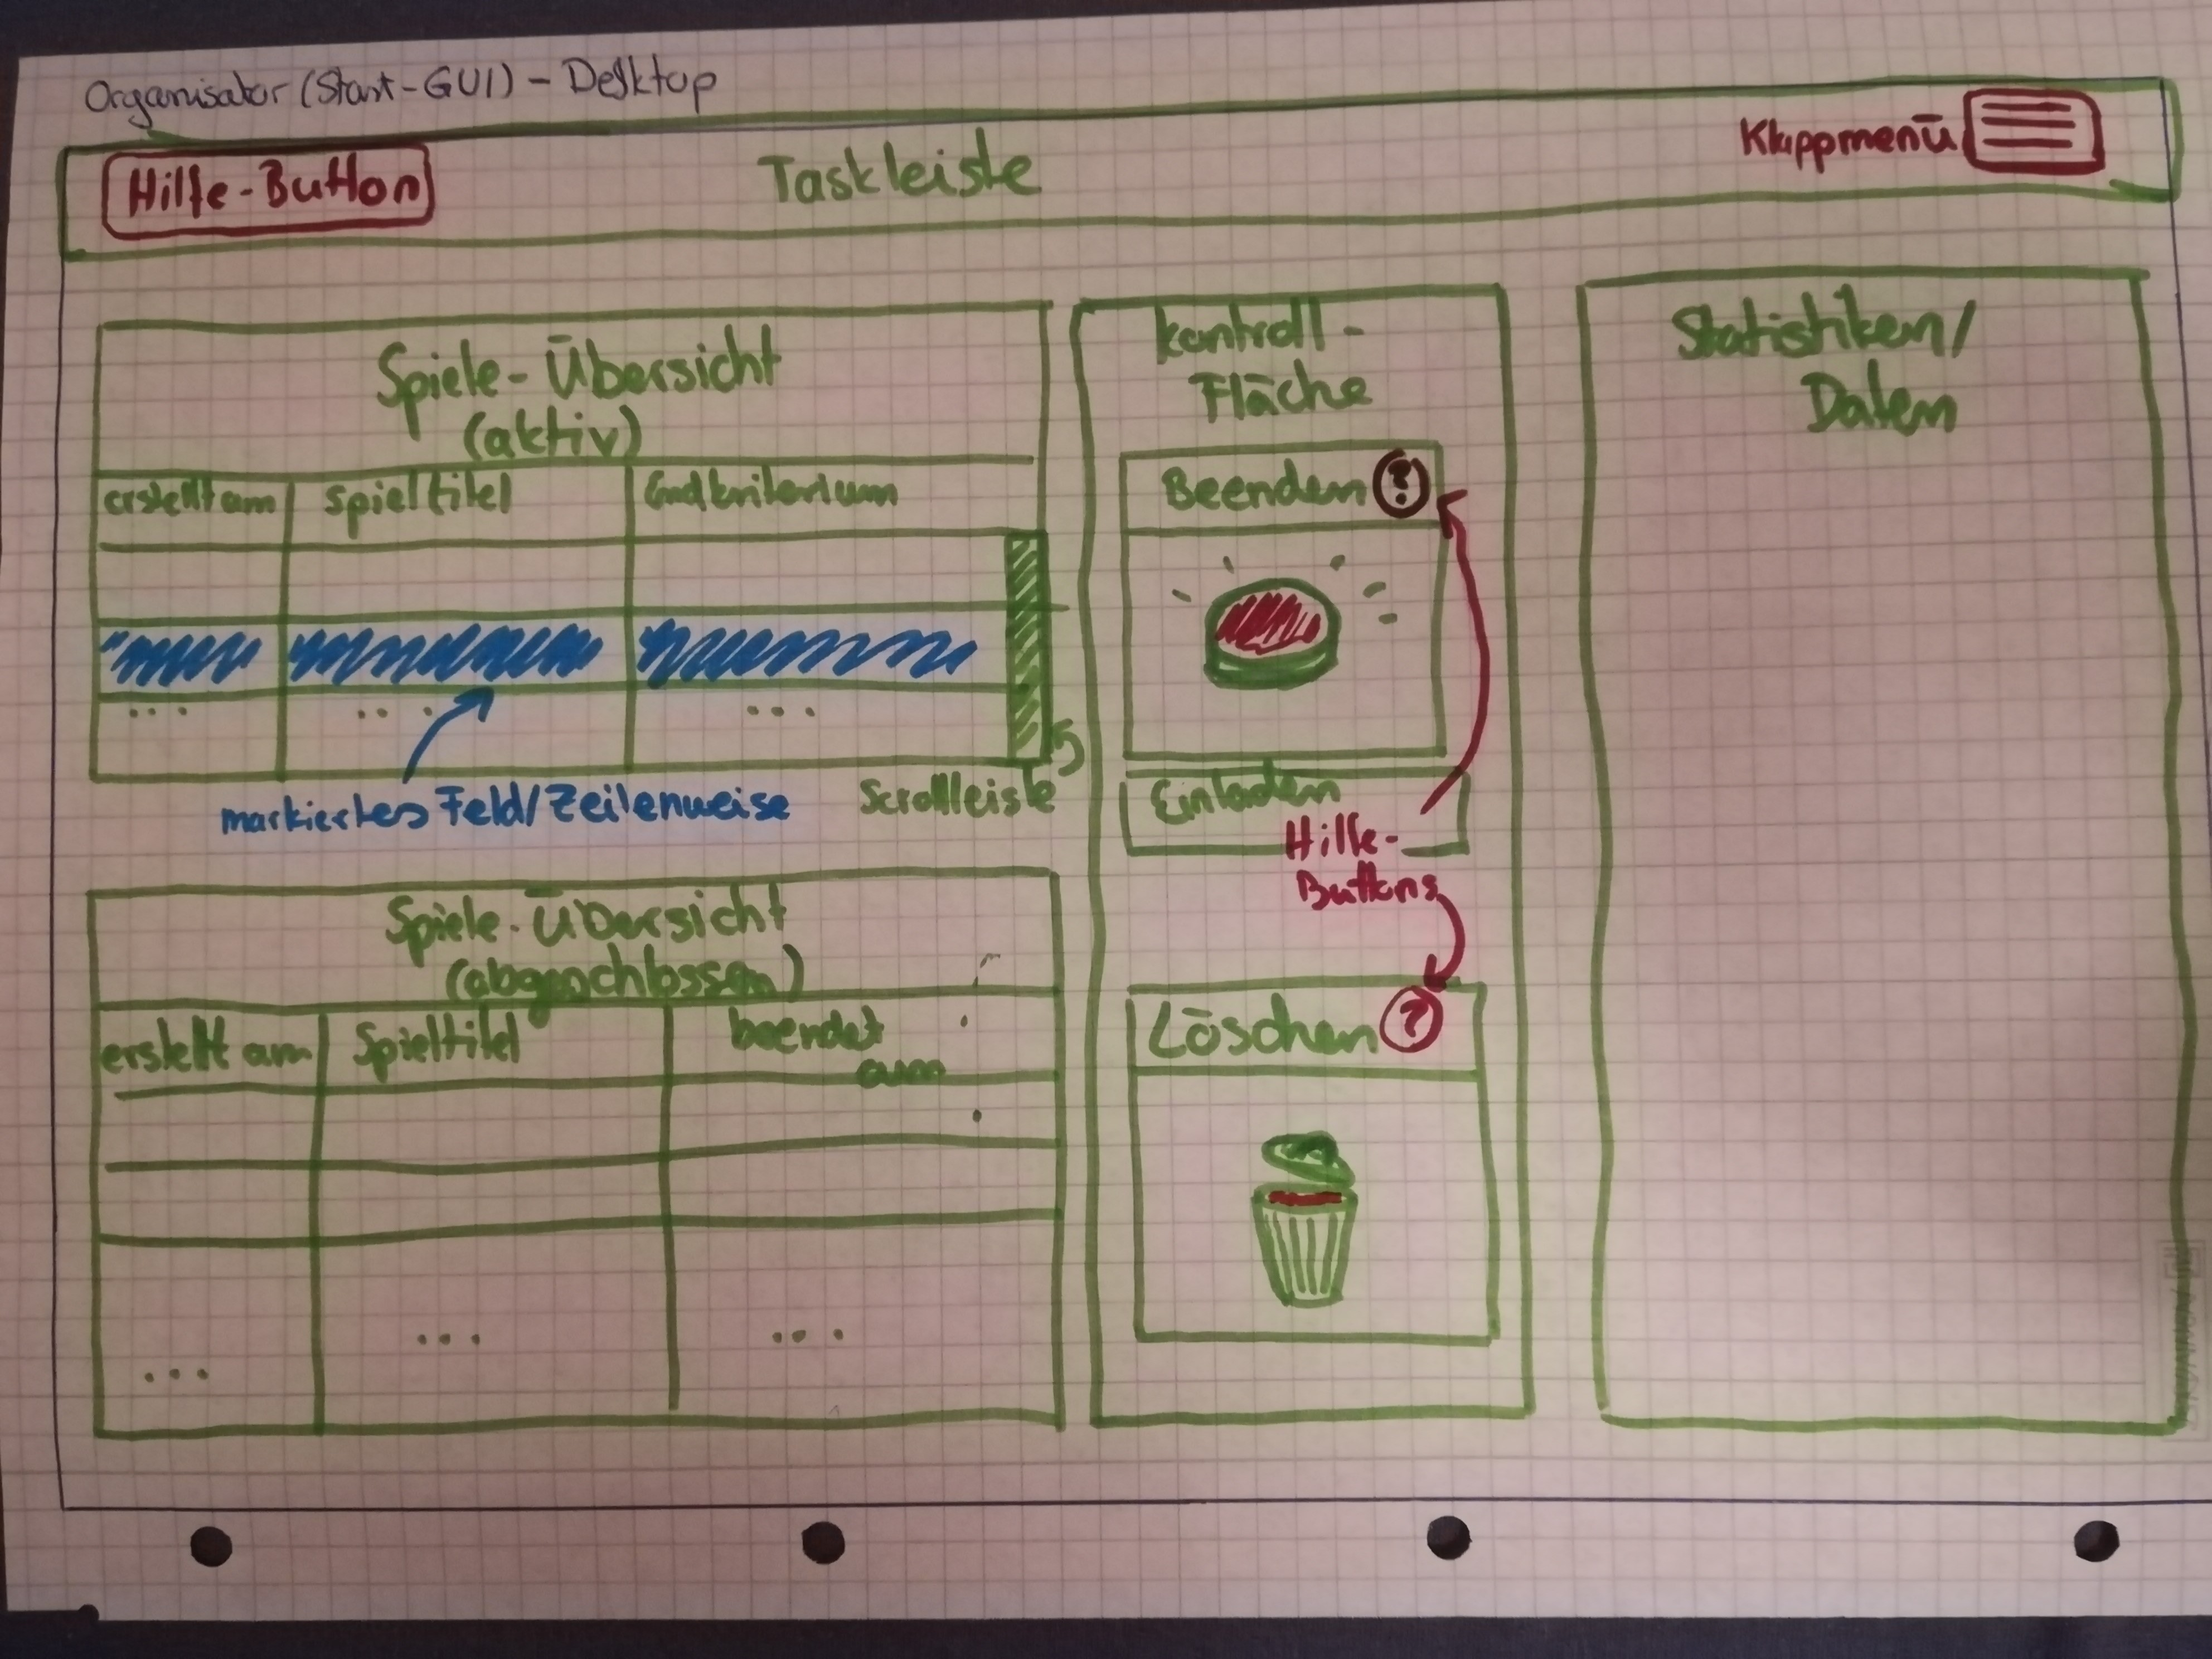
\includegraphics[width=\textwidth]{../pictures/2_Organisator.jpg}

    \subsection{Organisator-Start (responsive)}
    \centering
    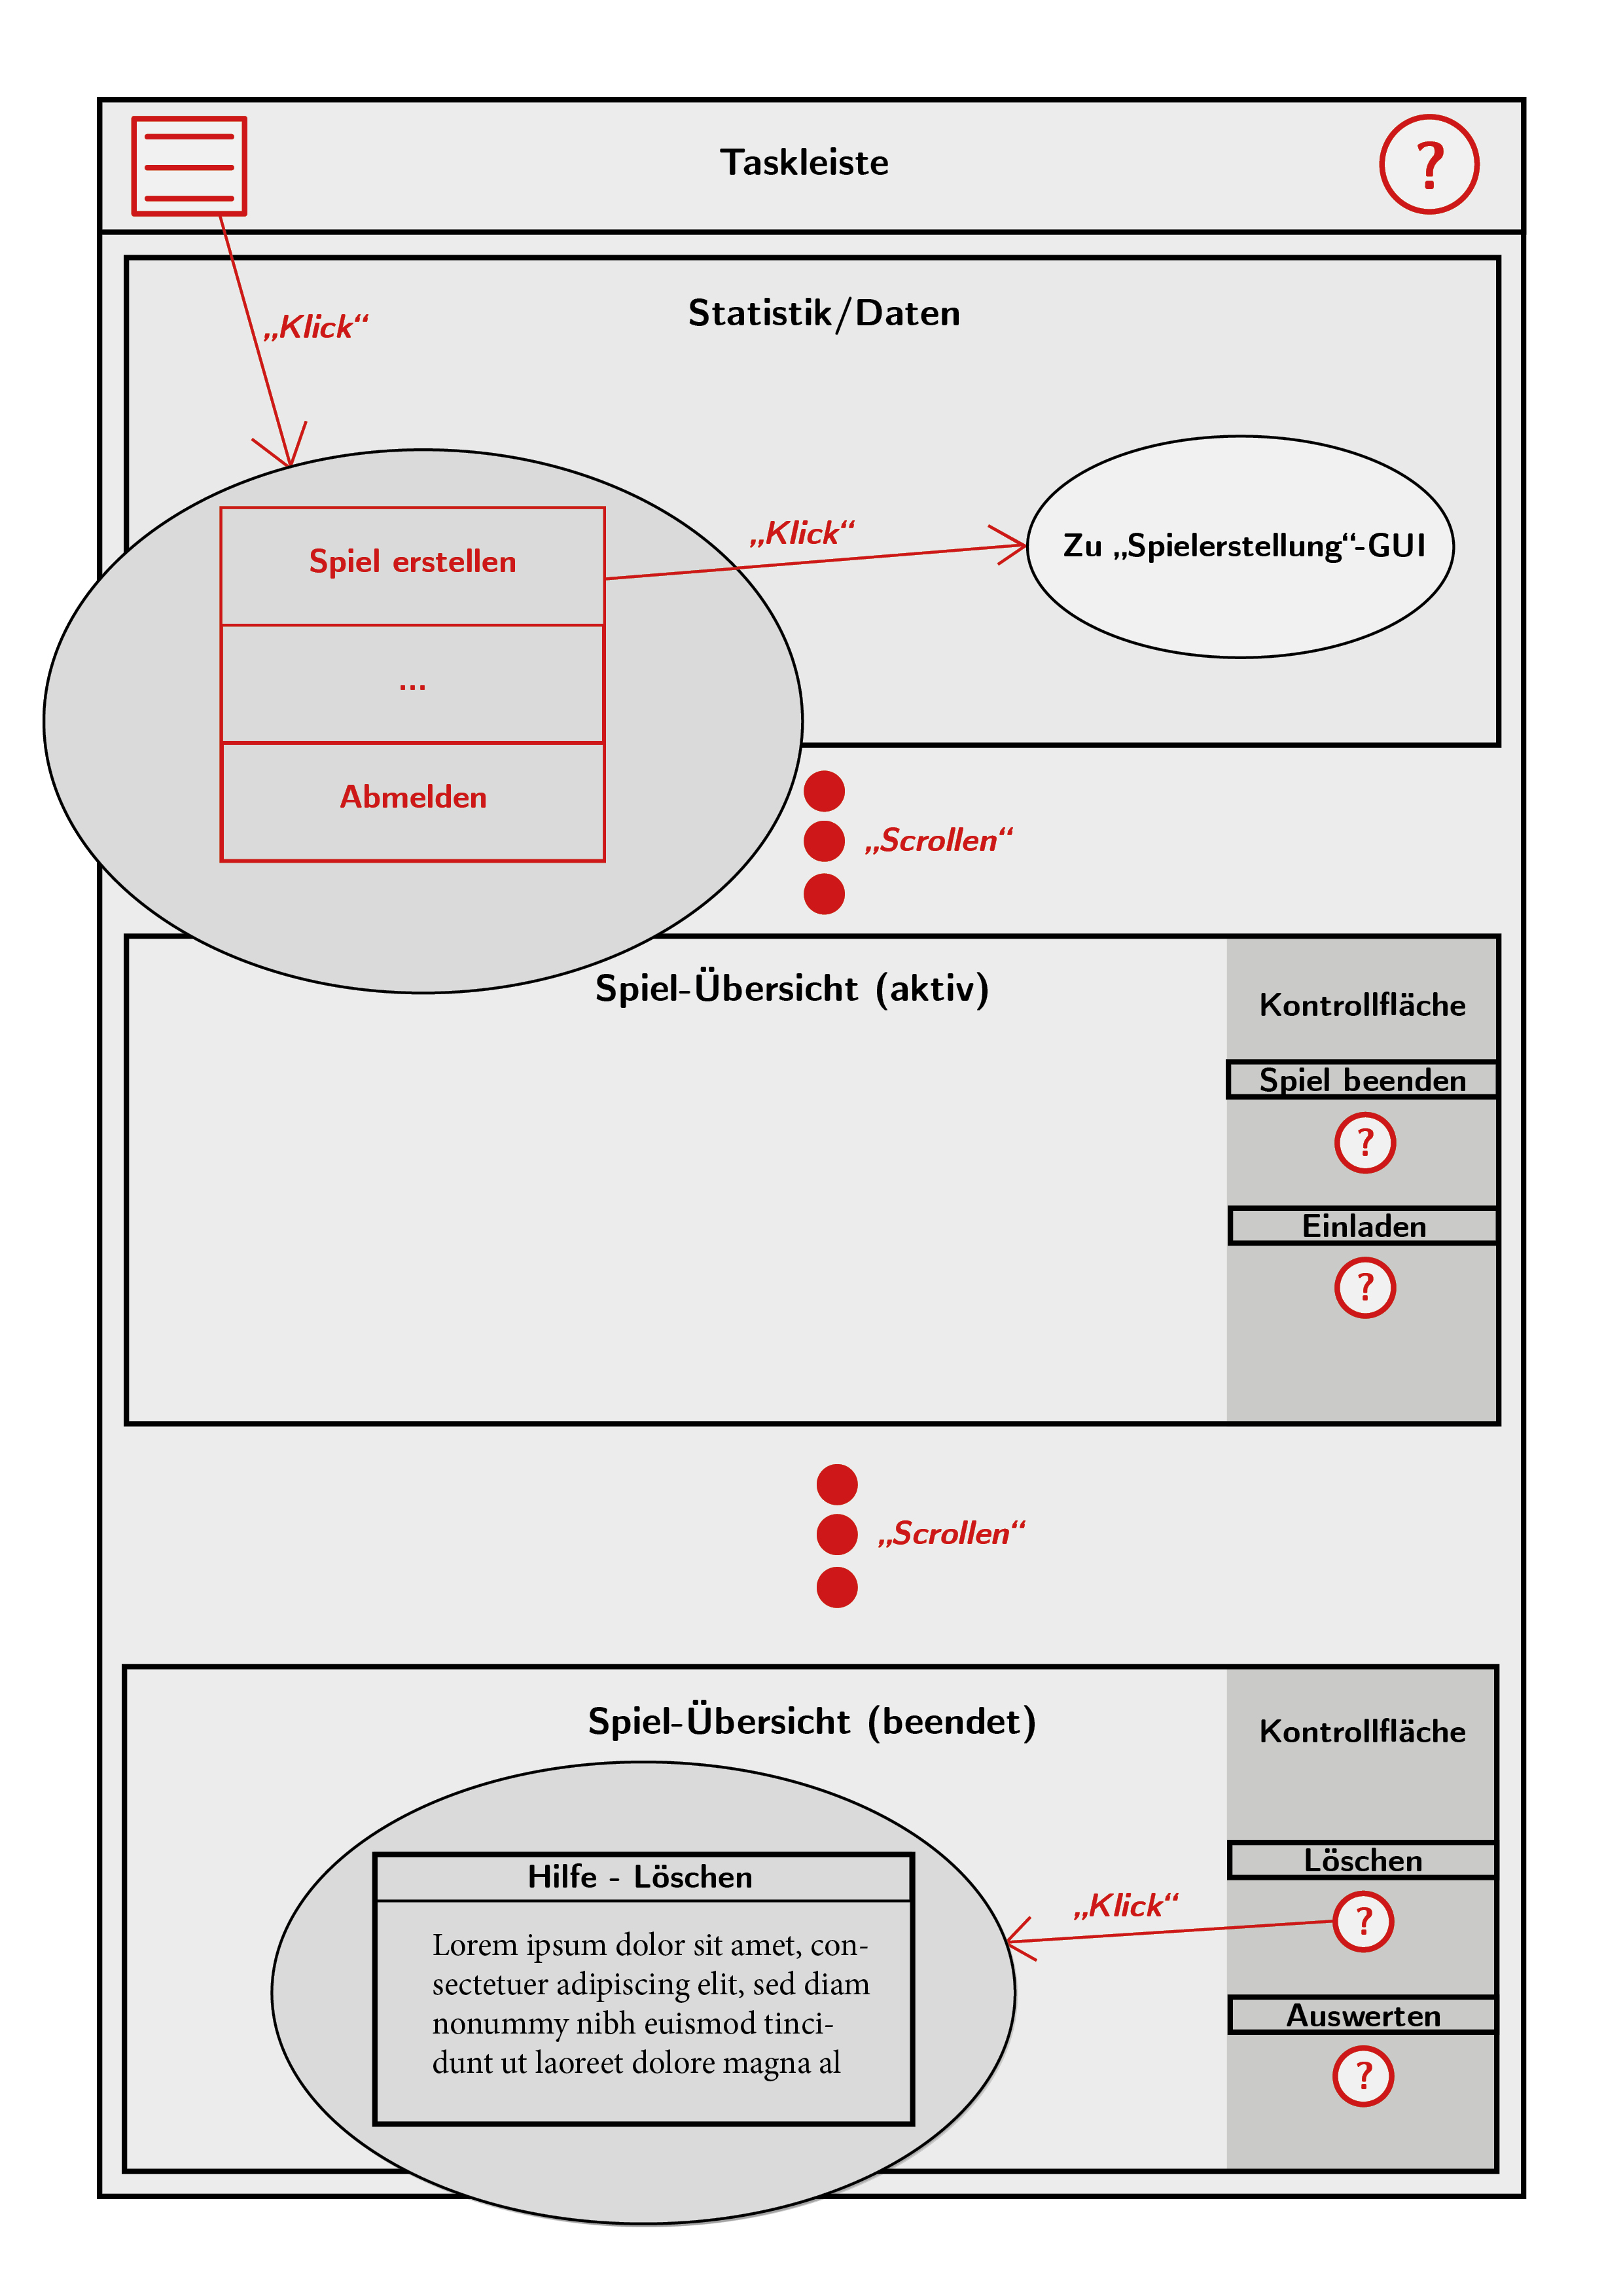
\includegraphics[width=\textwidth]{../pictures/3_Organisator(responsive).jpg}
    In den weiteren Darstellungen werden keine responsiven Darstellungen gezeigt, die zwei bereits gezeigten Darstellungen dienen als anschauliches Beispiel für
    responsive Darstellung einer Benutzerschnittstelle.

    \section{Spielerstellung}
    \centering
    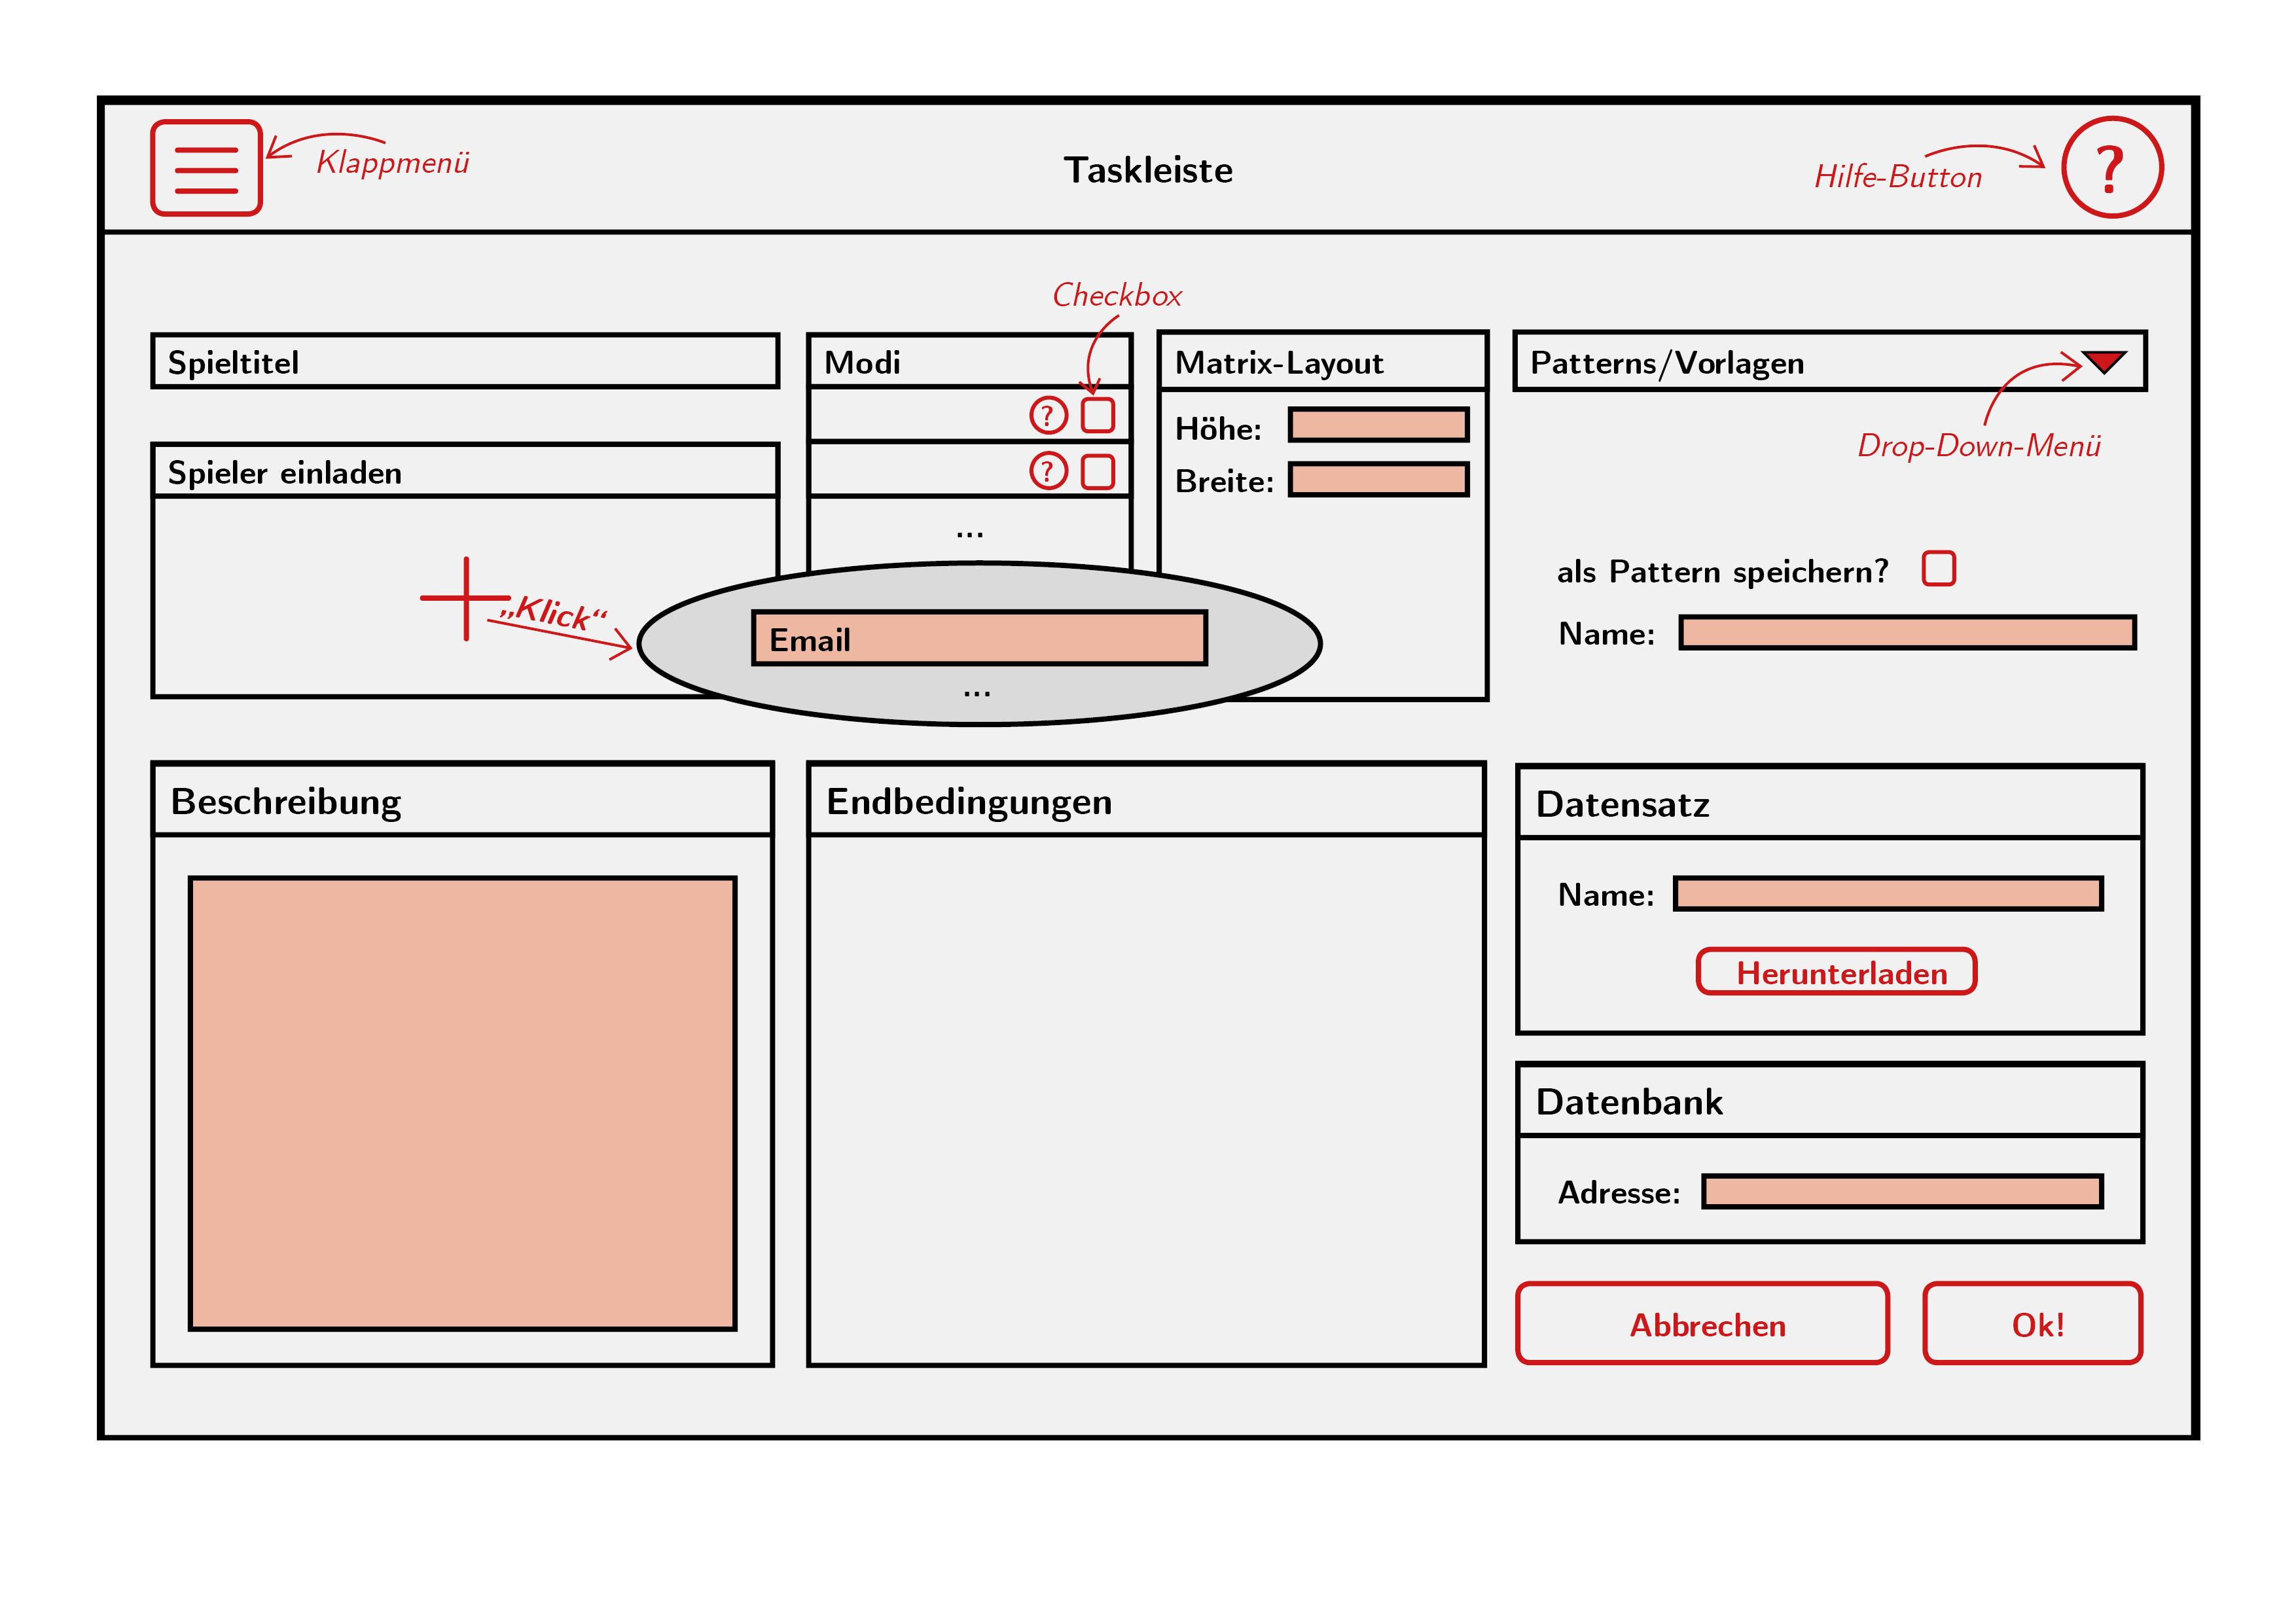
\includegraphics[width=\textwidth]{../pictures/Spielerstellung.jpg}

    \section{Spieler-Übersicht}
    \label{fig:Spieler-Übersicht}
    \centering
    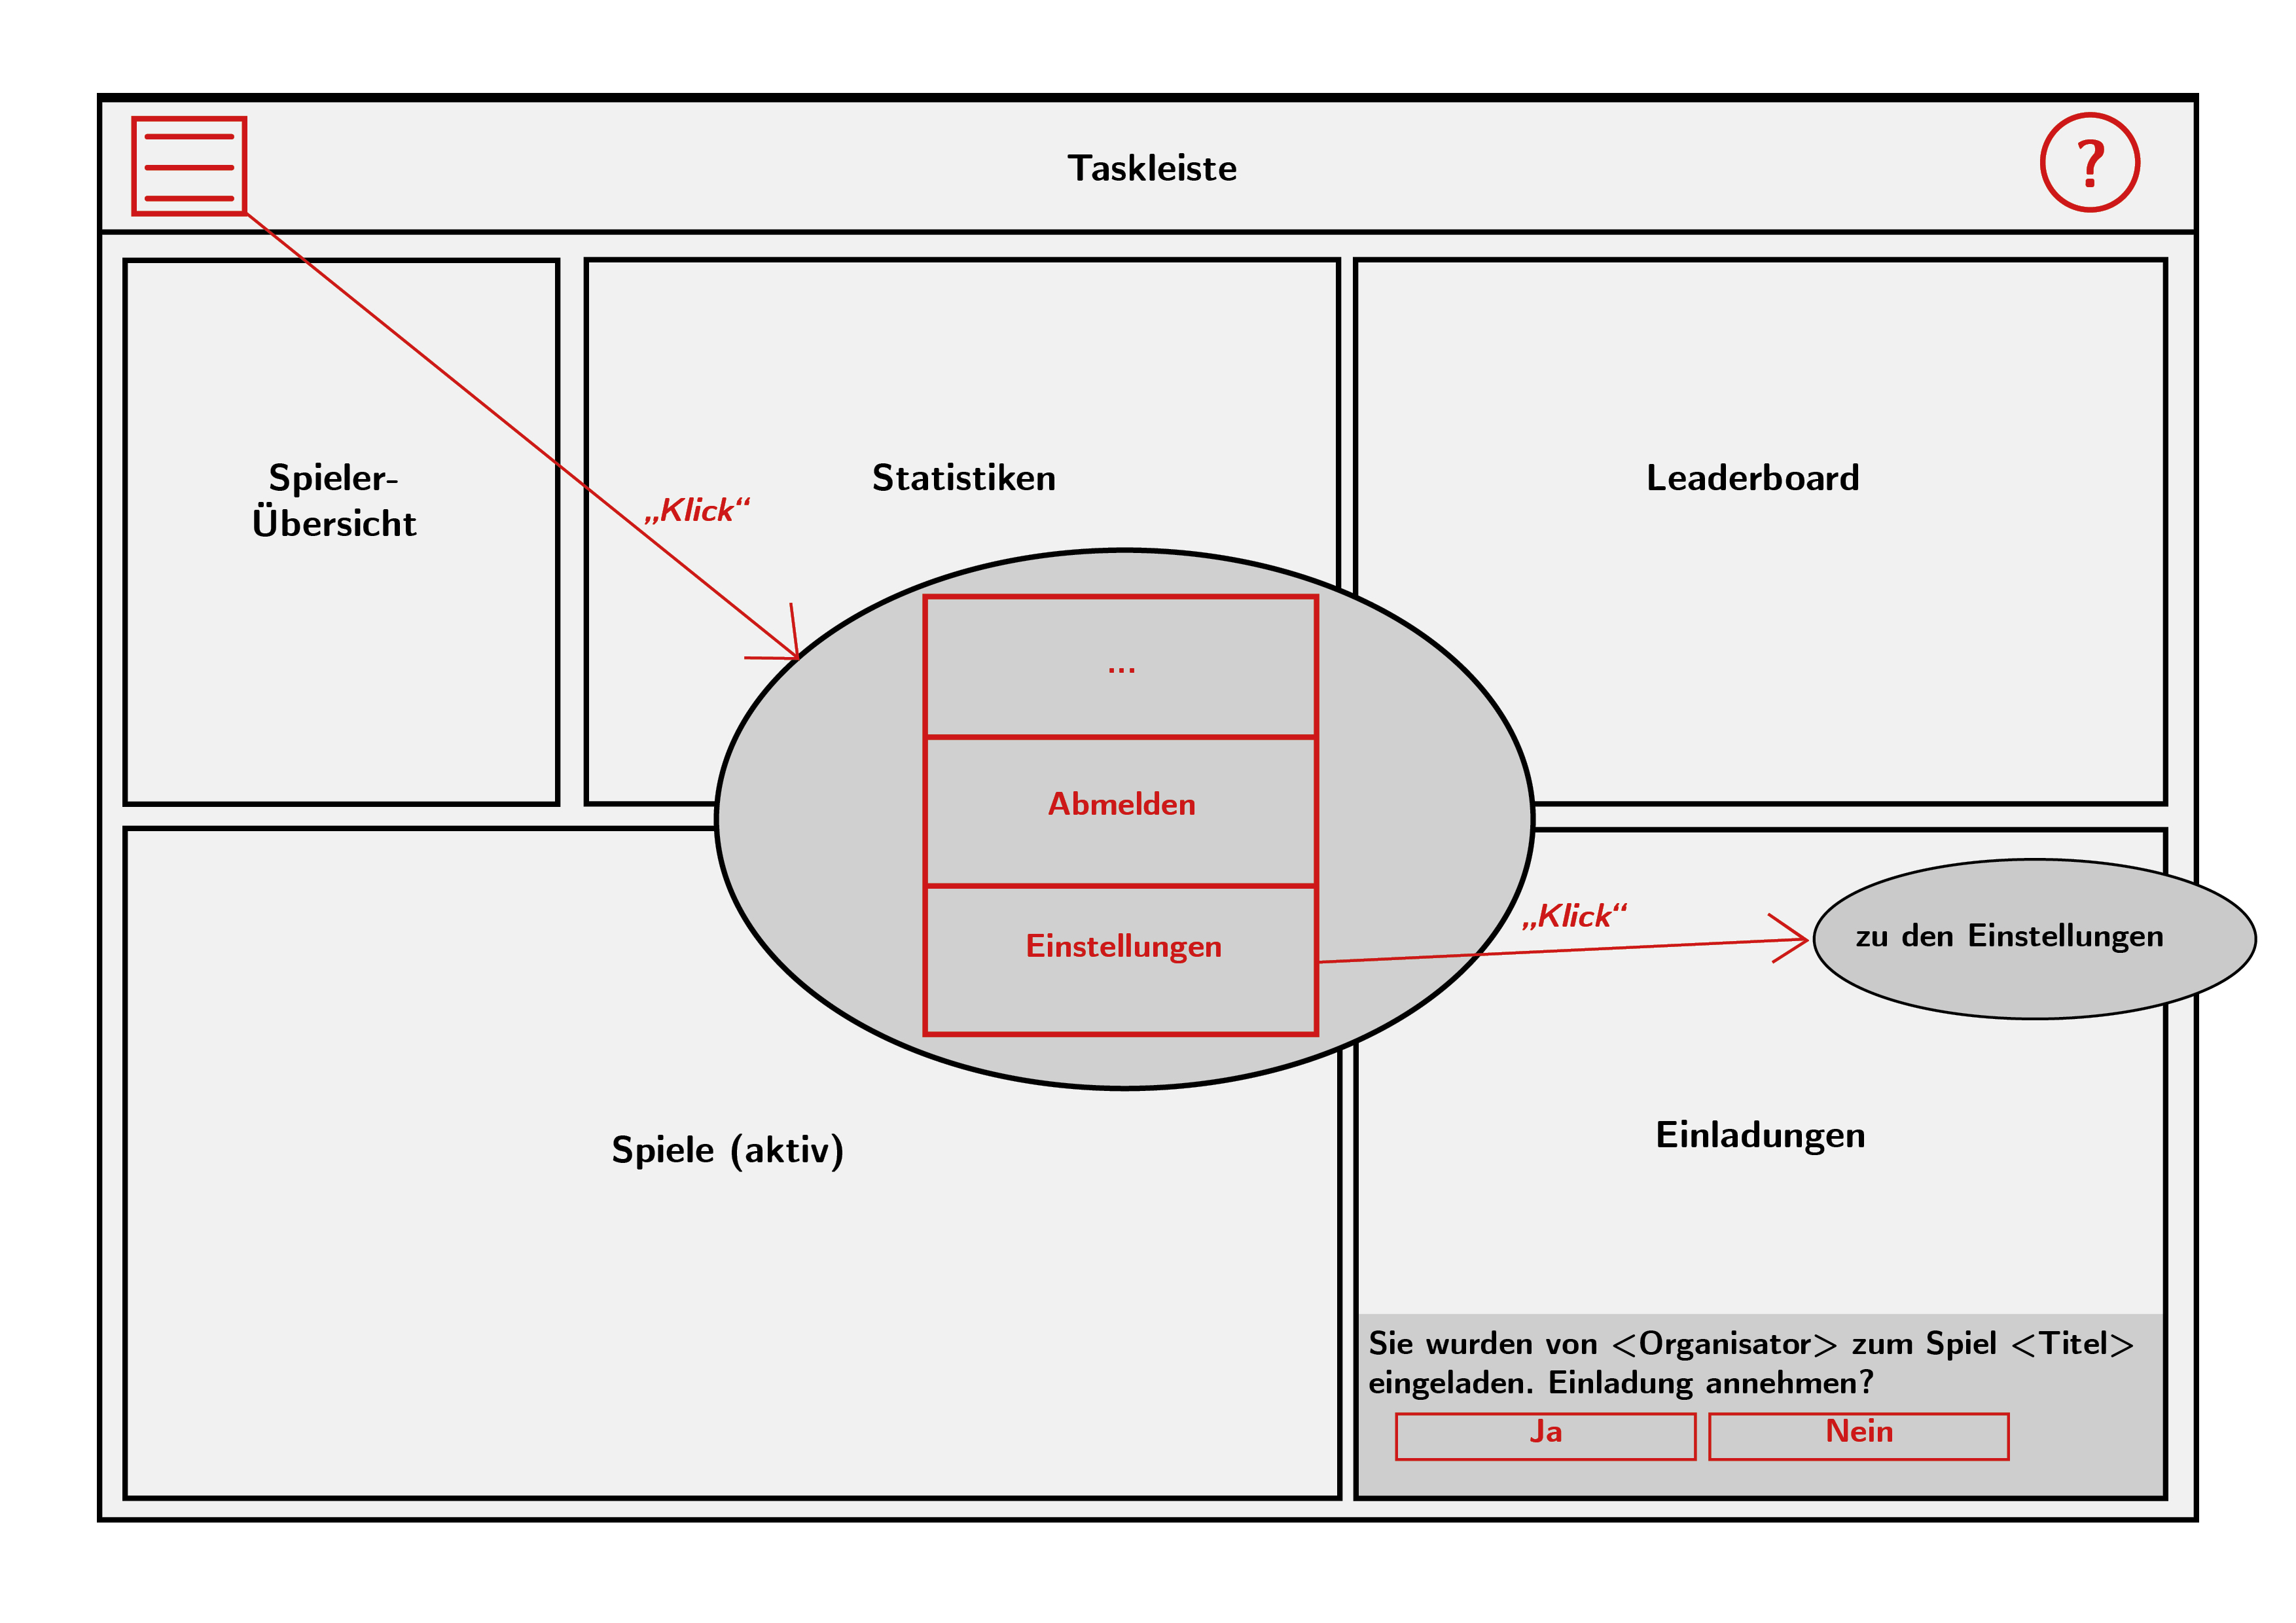
\includegraphics[width=\textwidth]{../pictures/5_Spieler.jpg}

    \section{Spiel}
    \subsection{Matrix Select}
    \centering
    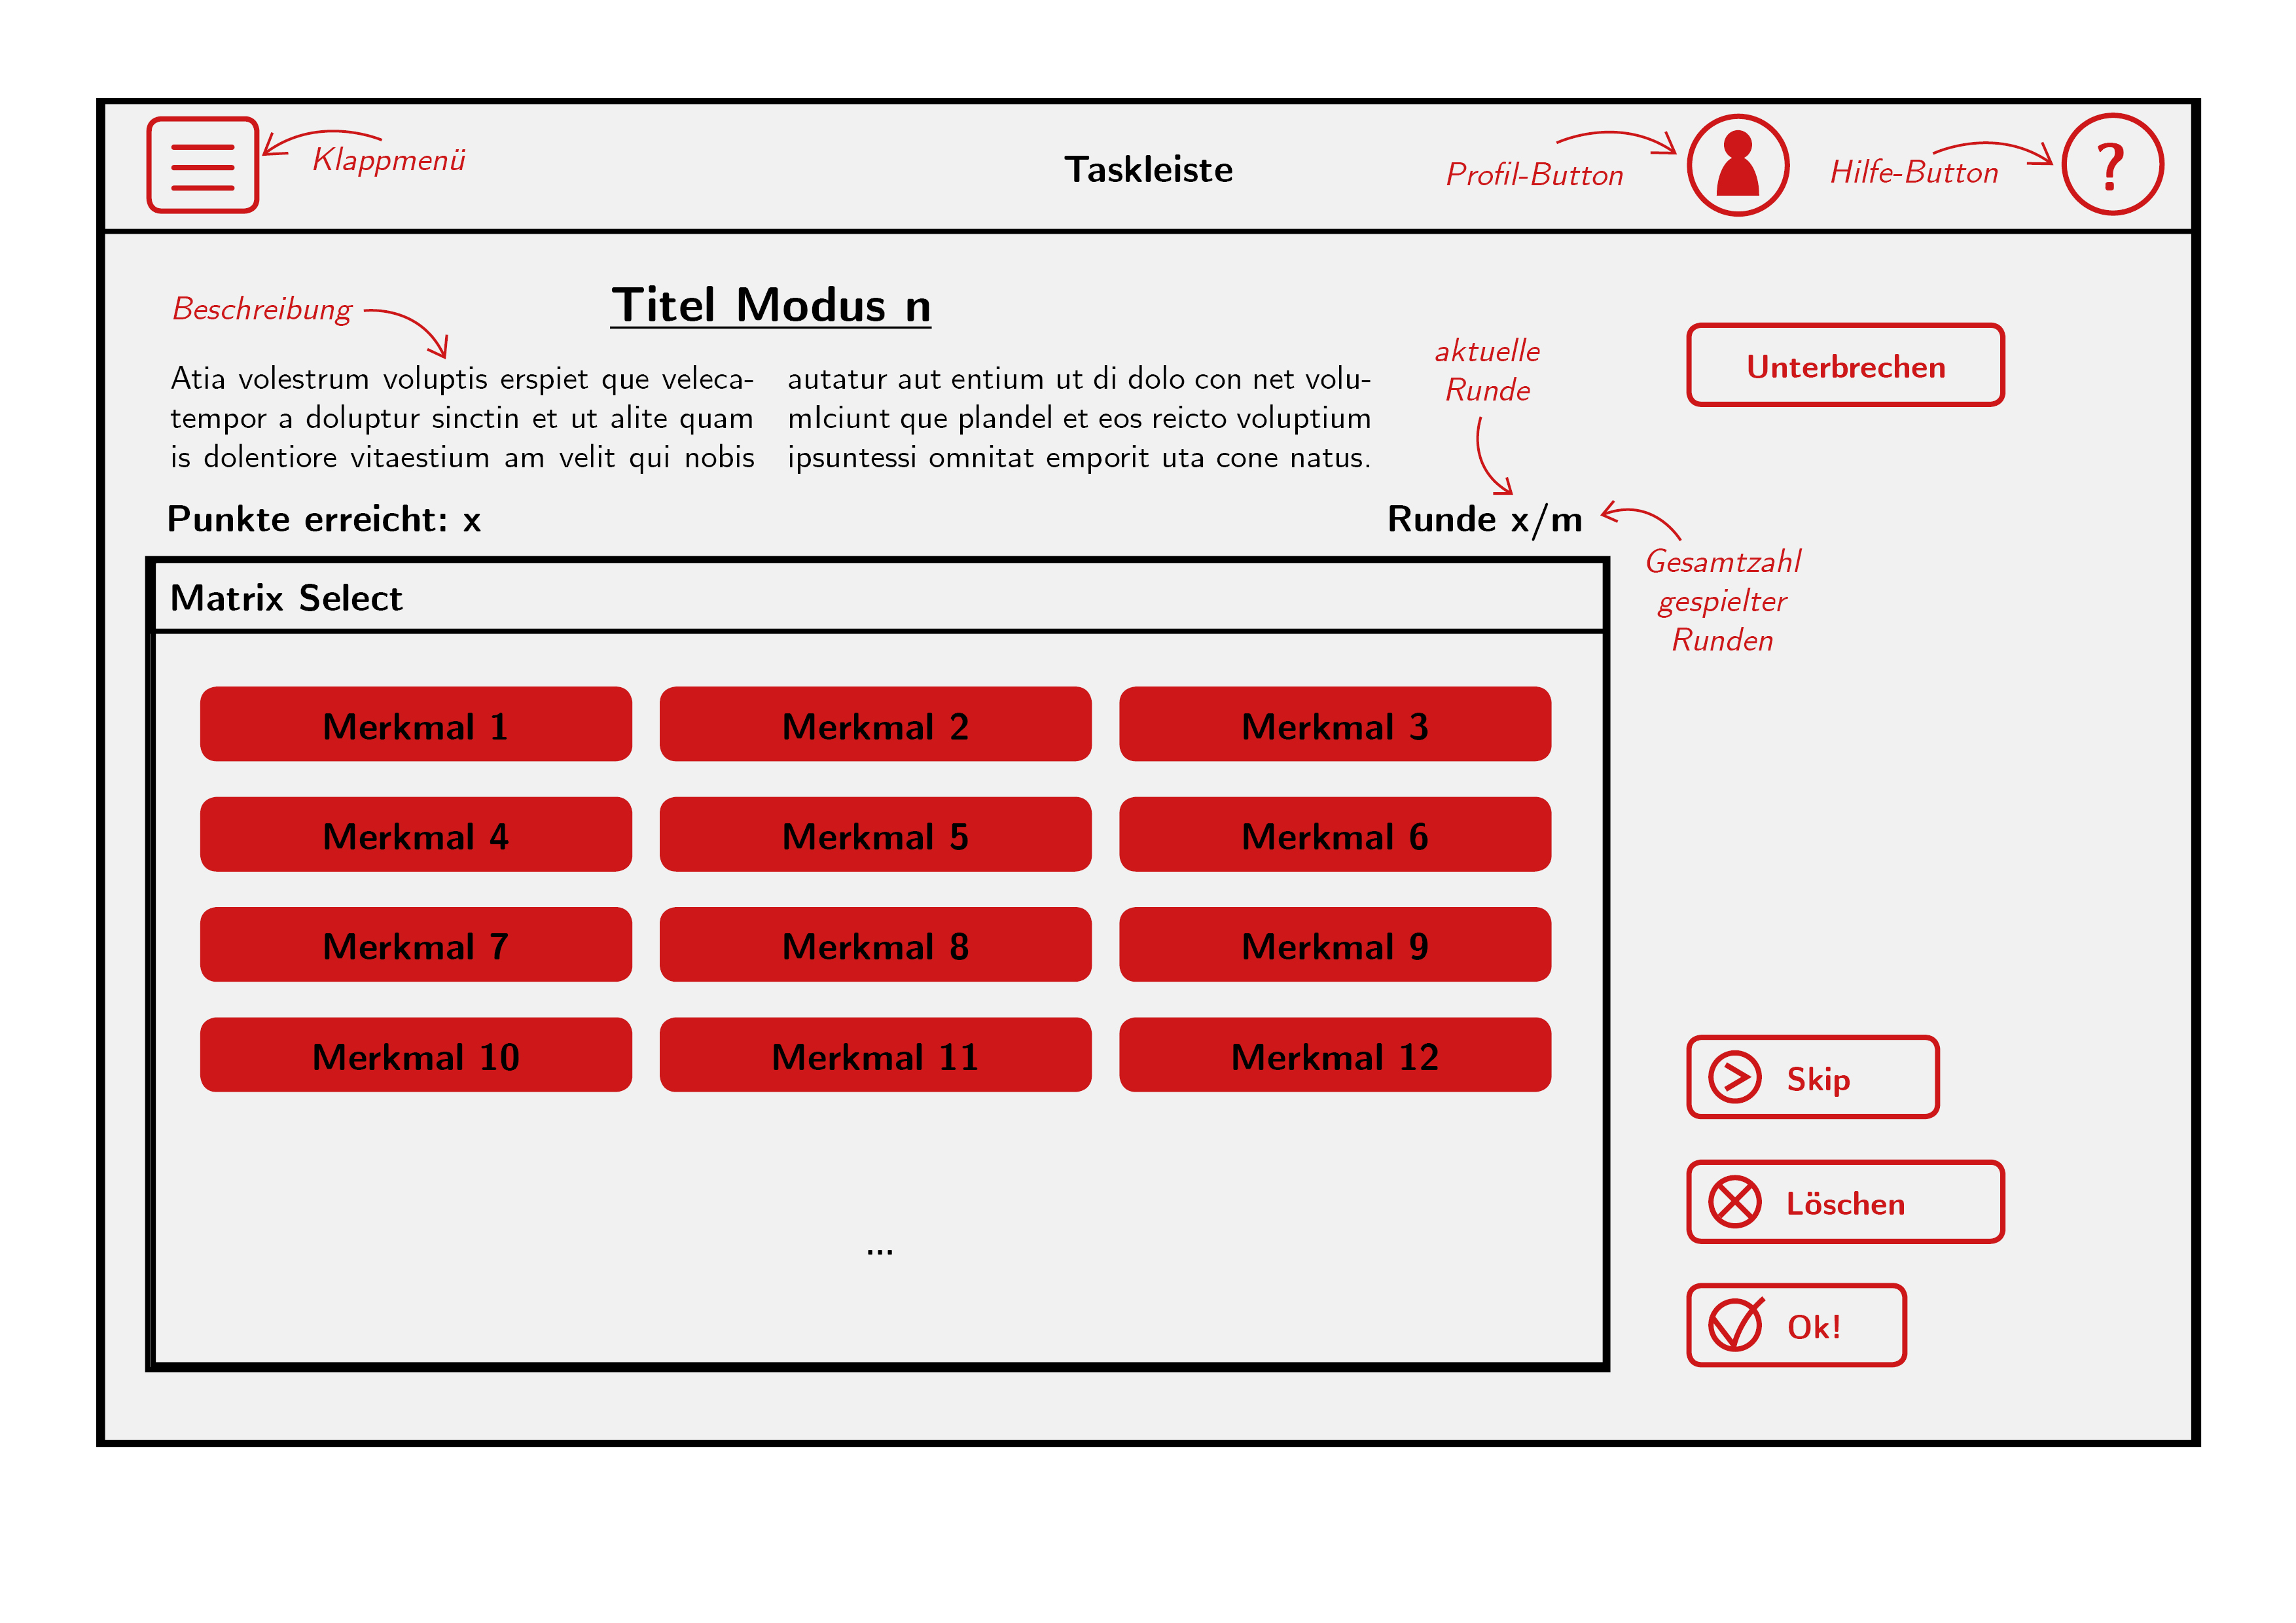
\includegraphics[width=\textwidth]{../pictures/MatrixSelect.jpg}
    \subsection{Binär Select}
    \centering
    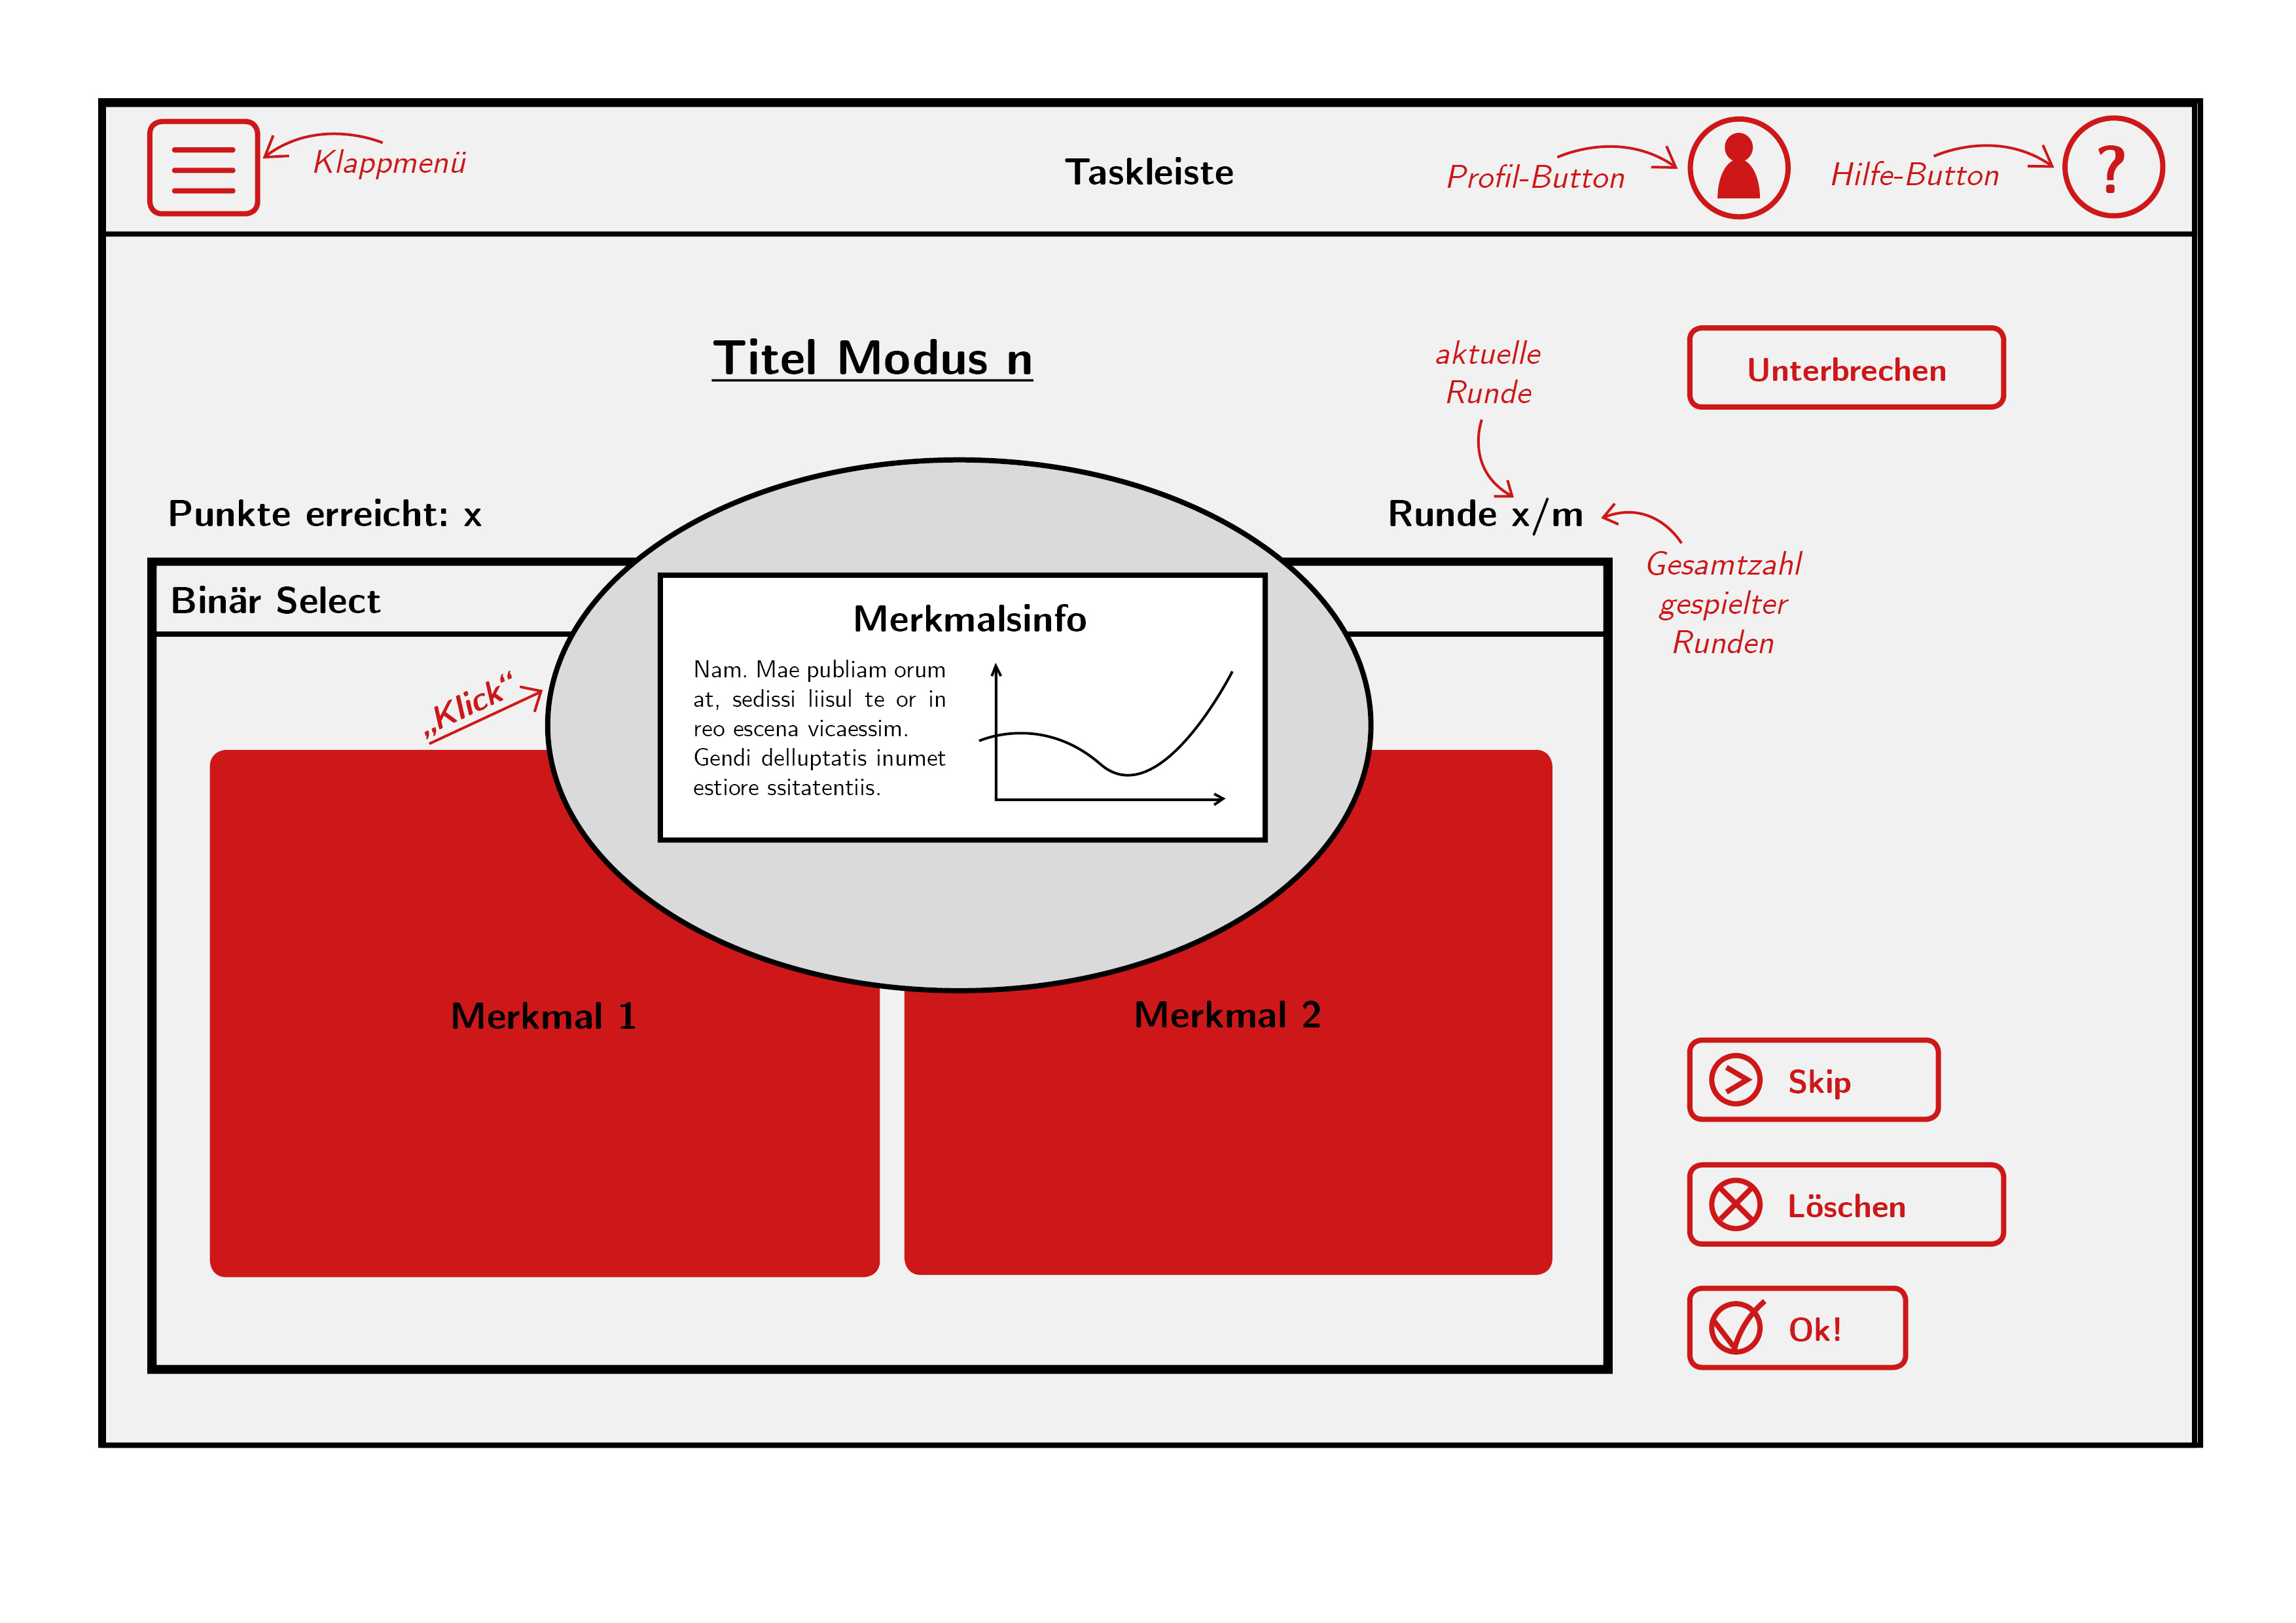
\includegraphics[width=\textwidth]{../pictures/BinSelect.jpg}

    \clearpage


    \chapter{Glossar}
    \printglossary
    \chapter{Anhang}
    \subsection{Auswahl an zu zeigenden Merkmalen}
    \label{fig:FeatureSelect}
    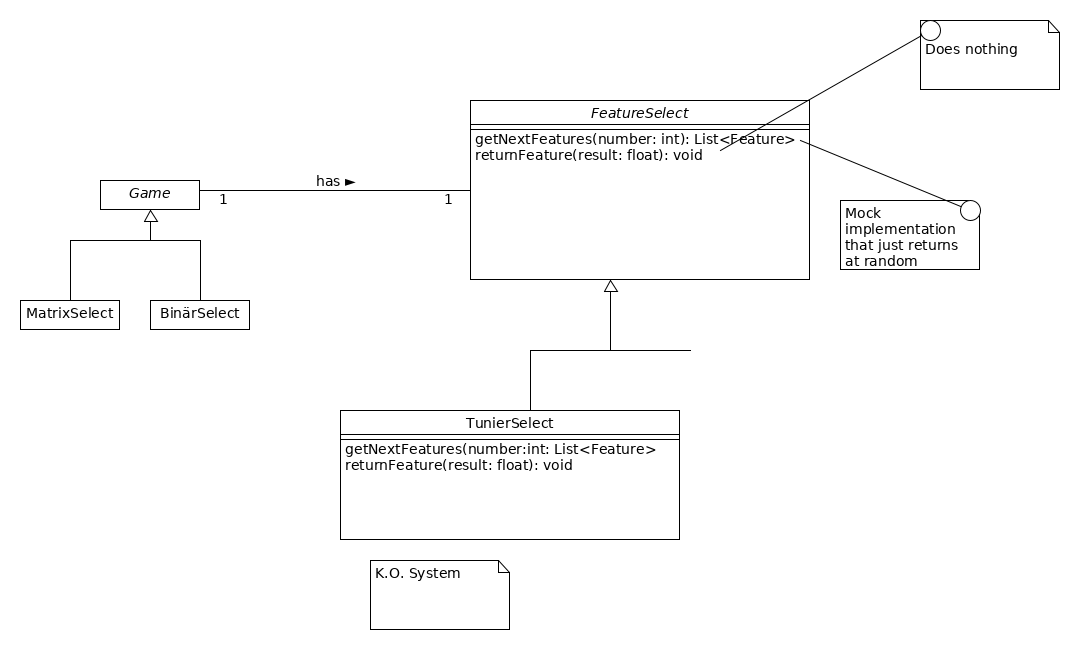
\includegraphics[width=\textwidth]{uml/export/FeatureSelect.png}
    
\end{document}
